\documentclass[a4paper]{article}\usepackage[]{graphicx}\usepackage[]{color}
% maxwidth is the original width if it is less than linewidth
% otherwise use linewidth (to make sure the graphics do not exceed the margin)
\makeatletter
\def\maxwidth{ %
  \ifdim\Gin@nat@width>\linewidth
    \linewidth
  \else
    \Gin@nat@width
  \fi
}
\makeatother

\definecolor{fgcolor}{rgb}{0.345, 0.345, 0.345}
\makeatletter
\@ifundefined{AddToHook}{}{\AddToHook{package/xcolor/after}{\definecolor{fgcolor}{rgb}{0.345, 0.345, 0.345}}}
\makeatother
\newcommand{\hlnum}[1]{\textcolor[rgb]{0.686,0.059,0.569}{#1}}%
\newcommand{\hlstr}[1]{\textcolor[rgb]{0.192,0.494,0.8}{#1}}%
\newcommand{\hlcom}[1]{\textcolor[rgb]{0.678,0.584,0.686}{\textit{#1}}}%
\newcommand{\hlopt}[1]{\textcolor[rgb]{0,0,0}{#1}}%
\newcommand{\hlstd}[1]{\textcolor[rgb]{0.345,0.345,0.345}{#1}}%
\newcommand{\hlkwa}[1]{\textcolor[rgb]{0.161,0.373,0.58}{\textbf{#1}}}%
\newcommand{\hlkwb}[1]{\textcolor[rgb]{0.69,0.353,0.396}{#1}}%
\newcommand{\hlkwc}[1]{\textcolor[rgb]{0.333,0.667,0.333}{#1}}%
\newcommand{\hlkwd}[1]{\textcolor[rgb]{0.737,0.353,0.396}{\textbf{#1}}}%
\let\hlipl\hlkwb

\usepackage{framed}
\makeatletter
\newenvironment{kframe}{%
 \def\at@end@of@kframe{}%
 \ifinner\ifhmode%
  \def\at@end@of@kframe{\end{minipage}}%
  \begin{minipage}{\columnwidth}%
 \fi\fi%
 \def\FrameCommand##1{\hskip\@totalleftmargin \hskip-\fboxsep
 \colorbox{shadecolor}{##1}\hskip-\fboxsep
     % There is no \\@totalrightmargin, so:
     \hskip-\linewidth \hskip-\@totalleftmargin \hskip\columnwidth}%
 \MakeFramed {\advance\hsize-\width
   \@totalleftmargin\z@ \linewidth\hsize
   \@setminipage}}%
 {\par\unskip\endMakeFramed%
 \at@end@of@kframe}
\makeatother

\definecolor{shadecolor}{rgb}{.97, .97, .97}
\definecolor{messagecolor}{rgb}{0, 0, 0}
\definecolor{warningcolor}{rgb}{1, 0, 1}
\definecolor{errorcolor}{rgb}{1, 0, 0}
\makeatletter
\@ifundefined{AddToHook}{}{\AddToHook{package/xcolor/after}{
\definecolor{shadecolor}{rgb}{.97, .97, .97}
\definecolor{messagecolor}{rgb}{0, 0, 0}
\definecolor{warningcolor}{rgb}{1, 0, 1}
\definecolor{errorcolor}{rgb}{1, 0, 0}
}}
\makeatother
\newenvironment{knitrout}{}{} % an empty environment to be redefined in TeX

\usepackage{alltt}
\usepackage[utf8]{inputenc}
\usepackage[T1]{fontenc}
\usepackage{amsfonts}
\usepackage[sectionbib]{natbib}
\usepackage{graphicx}
\usepackage{lmodern}
\usepackage{amssymb,amsmath}
\usepackage{xcolor}
\usepackage{booktabs}
\usepackage{longtable}
\usepackage{array}
\usepackage{multirow}
\usepackage{wrapfig}
\usepackage{float}
\usepackage{colortbl}
\usepackage{pdflscape}
\usepackage{tabu}
\usepackage{threeparttable}
\usepackage{threeparttablex}
\usepackage[normalem]{ulem}
\usepackage{makecell}
\usepackage[margin=1in]{geometry}

\bibliographystyle{tpb}
\newcommand{\adata}{\ensuremath{\mathcal{D}}}
\newcommand{\data}{\ensuremath{D}}
\newcommand{\datab}{\ensuremath{D_{b}^*}}
\newcommand{\databb}{\ensuremath{D_{bc}^{**}}}
\newcommand{\boo}[1]{\ensuremath{{#1}_{b}^{*}}}
\newcommand{\CDF}{\ensuremath{\mathrm{CDF}}}
\newcommand{\sfn}{\ensuremath{\mathrm{s}}}
\newcommand{\tfn}{\ensuremath{\mathrm{t}}}
\newcommand{\bth}{\ensuremath{\boldsymbol{\theta}}}
\newcommand{\bSigma}{\ensuremath{\boldsymbol{\Sigma}}}
\DeclareMathOperator{\Esp}{E}

\title{Supplementary Information for}
\usepackage{etoolbox}
\makeatletter
\providecommand{\subtitle}[1]{% add subtitle to \maketitle
  \apptocmd{\@title}{\par {\large #1 \par}}{}{}
}
\makeatother
\subtitle{Lower fertility for mothers with higher twinning propensity in pre-industrial Europe}
\author{I. J. Rickard \and C. Vullioud \and F. Rousset \and E. Postma \and S.
Helle \and V. Lummaa \and R. Kylli \and J. E. Pettay \and E.
Røskaft \and G. R. Skjærvø \and C. Störmer \and E. Voland \and D.
Waldvogel \and A. Courtiol\footnote{corresponding author: courtiol@izw-berlin.de}}

\date{}
\IfFileExists{upquote.sty}{\usepackage{upquote}}{}
\begin{document}

\renewcommand{\thetable}{S\arabic{table}}
\renewcommand{\thefigure}{S\arabic{figure}}



\maketitle

\tableofcontents

\newpage

\listoffigures

\newpage

\listoftables

\newpage

% \section{Section 1: the heterogeneity hypothesis and the Utah population}
%
% In 2011, \citeauthor{Robson2011} published a paper advancing the so-called heterogeneity hypothesis: "Twinning may be an indicator of higher maternal capacity and may identify those women whose enhanced phenotypic quality allows them to bear these elevated reproductive costs". As \citet{Rickard2012} argued however, all the predictions from  \citet{Robson2011} suffer from a key methodological issue that casts doubt on this finding. Because \citet{Robson2012} repudiated this criticism, we here unpack their arguments as well as ours for readers interested in the specific controversy.
%
% That individuals may evolve mechanisms to modulate the expression of their traits according to their phenotypic quality is not questioned. This is true irrespective of whether one defines phenotypic as a source of fixed or dynamic heterogeneity between individuals. In fact, this idea has been the focus of thousands of studies performed in a myriad of species. This includes for instance studies from the field of behavioural ecology known as condition dependence. That phenotypic quality has shaped the evolution of a given trait is however particularly difficult to demonstrate. One main difficulty is that it is not clear what the phenotypic quality (or condition) really is, how to define it, and how to measure it \citep[e.g.][]{Cotton2004, Wilson2010}. Another, as \citet{Robson2011} pointed out, is that variation in phenotypic quality is overlaid on top of trade-offs in resource allocation. Indeed, when resource acquisition varies between individuals, inferring trade-offs from phenotypic correlations is in itself difficult \citep[e.g.][]{VanNoordwijk1986, Pease1988, Bolund2020}.
%
% \citet{Robson2011} thus decided not to test the effect of phenotypic quality as such but to test predictions consistent with their heterogeneity hypothesis. Namely, that "twinning mothers should exhibit additional features of a robust phenotype, including shorter average inter-birth intervals, later ALB [age at last birth] and longer reproductive spans resulting in higher parities, and longer postmenopausal lifespans". The outputs of their statistical analyses comparing these variables between twinners and non-twinners were consistent with the predictions the authors made, which led them to conclude that the heterogeneity hypothesis must be right. \citet{Rickard2012}'s concern is that the same predictions would hold even if the specific heterogeneity hypothesis considered by \citet{Robson2011} does not hold.
%
% \citet{Rickard2012} argued that all the predictions from \citet{Robson2011} related to the relationship between twinning and fertility suffer from a key methodological issue: they are framed in terms of problematic comparisons between mothers that produced twins and mothers that did not. Such comparisons are problematic because differences related to fertility are expected to be found between twinners and non twinners irrespective of the presence or absence of heterogeneity in the phenotypic quality of mothers. This is because twinners and non-twinners do not just differ from a difference in their twinning propensity, but they also differ in their exposure to the risk of twinning \citep[see][and Discussion in main text for illustrations]{Rickard2012}. Even if the patterns predicted by \citet{Robson2011} are correct, we do not need the heterogeneity between mothers to cause it. In fact, it suffices to reverse the causality of the predictions to see that a different mechanism as the one proposed by \citet{Robson2011} may also be consistent with the observations:
%
% \begin{itemize}
% \item do twinners have shorter interbirth intervals because they are of higher quality, or do women that have shorter interbirth intervals are more likely to get twins because they give birth more times?
% \item do twinners have a later age at last birth or a longer reproductive span because they are of higher quality, or do women that have a later age at last birth or a longer reproductive span are more likely to get twins because they give birth more times?
% \item do twinners have more births because they are of higher quality, or do women that have more births are more likely to get twins precisely because they play the "twin lottery" more times.
% \end{itemize}
%
% The situation for postmenopausal lifespan is different since this prediction does not relate to differences in fertility between mothers and therefore does not concern us here.
%
% That predictions about difference between twinners and non-twinners may hold irrespective of the true direction of the causality reaches beyond the traditional "correlation does not imply causation" issue. Indeed, here the problem is that predictions made by \citet{Robson2011} may be validated irrespective of the veracity of their hypothesis. Worse, the predictions obtained by reversing causality are not the product of some unlikely hypothesis but an unavoidable statistical consequence (the more you play the lottery, the more likely you are to win). This means that once the causality is reversed, the predictions will hold (e.g. mothers that would produce more birth due to chance alone would also be more likely to end up being classified as twinners) whether the heterogeneity hypothesis (or indeed, other forms of condition dependence) hold or not.
%
% In their comment, \citet{Rickard2012} also presented the result of a very simple simulation study illustrating the issue. The simulation experiment showed that even when the heterogeneity hypothesis does not apply (something that \citet{Rickard2012} implemented by assuming that the twinning propensity was the same across all mothers), analysing the data generated by comparing twinners and non-twinners yielded in results which were both qualitatively and quantitatively similar to those presented by \citet{Robson2011}. In other words, they obtained results that are typically interpreted as supportive of the heterogeneity hypothesis, although the simulations, by construction, did not emulate any of the mechanisms which the hypothesis assumes.
%
% Importantly, the message of \citet{Rickard2012} comment was not to suggest that the heterogeneity hypothesis does not apply to the Utah population studied by \citet{Robson2011} -- a point which we will return to below. Instead, \citet{Rickard2012}'s conclusion was that the predictions and analyses performed by \citet{Robson2011} were not suitable to test the heterogeneity hypothesis.
%
% In reply to \citet{Rickard2012} comments. \citet{Robson2012} criticised the simulation study made by  \citet{Rickard2012} and presented new results aimed to support their initial finding. Concerning the simulation study, \citet{Robson2011} questioned the simplicity of the assumptions made by  \citet{Rickard2012} to generate their synthetic data. They remarked that \citet{Rickard2012} did not consider the higher infant mortality rate of twins compared to singletons and its negative effect on the duration of interbirth intervals. They also criticised that \citet{Rickard2012} did not consider that the twinning propensity varies with the age of mothers. However, this has no bearing on the logical argument of \citet{Rickard2012}. The simulation showed that even in the absence of heterogeneity between mothers, twinners are expected to have more children. Considering that the death of twin infants may reduce interbirth intervals should in fact increase the apparent higher fertility of mothers with twins; but, like the effect of mother's age, those details have nothing to do with what the simulation demonstrated; namely, that comparing twinners and non-twinners can lead to misleading conclusions.
%
% The simulations presented in the main text of the current paper are different from those made by \citet{Rickard2012}. This time, the simulations do not fall into the category of proof-of-concept models \citep{Servedio2014}. Instead, they are used to compare different mechanisms based on the quantitative relationship they create between twinning propensity of the total number of births. For this reason, the life history of the virtual individuals is simulated with much more realism. In particular, all the details mentioned by \citet{Robson2012} are now considered. That twinners may have shorter interbirth intervals after giving birth to twins is modeled by mechanism B (see main text; yet again it is not necessary to model explicitly why this occurs -- the death of the infants may be one of the reasons). That the twinning propensity varies with the age of the mothers is modelled by mechanism C.
%
% We now turn to the analyses presented in \citet{Robson2012}. All the new results focused on the analysis of parity progression ratios. They "compared the proportion of twinning mothers who bear an additional child relative with non-twinning mothers at that same parity" and found that twinners have higher parity progression ratios at any parity (at least in the earlier cohort). Unfortunately, this additional analysis does not cope with our main criticism since twinners are still compared to non-twinners. Again, it is easy to reverse the causality to show that the predicted patterns hold in the absence of the specific heterogeneity hypothesis they considered:
%
% \begin{itemize}
% \item do twinners have higher parity progression because they are of higher quality, or do mothers that have higher parity progression are more likely to get twins because they give birth more times?
% \end{itemize}
%
% Had \citet{Robson2012} analysed non-aggregated data with the value of the variable representing the outcome of twinning being defined for the parity considered instead of being defined across all births a mother gave to, the answer would have been clear. In addition to presenting the results of a comparison of the mean parity progression ratios between twinners and non-twinners, they also presented the results as a ratio and as an odds-ratio. Unfortunately, using means, ratios, odd-ratios, or whichever metric, has no relevance to the problem. The same is also true of the statistical model used and the covariates considered in the analysis: as long as twinning status is defined over the full life history of the mothers, twinners and non-twinners do not simply differ by their twinning propensity but also by their realised fertility which confounds the results. In sum, none of the arguments put forward by \citeauthor{Robson2012} in their 2012 reply addresses the fundamental issue pointed by \citet{Rickard2012}.
%
% In conclusion, until the right analyses are done on the data from historical Utah, one simply cannot tell if, as we found for our European data, the heterogeneity hypothesis should be rejected, or if the hypothesis is likely to be correct in that population. Other studies have shown that the Utah population shows different biological characteristics from European populations it originated from -- a result that may be explained by the particular history of the demography of this pioneer population. For example, the variance in relative fitness increased during the demographic transition in Utah \citep{Moorad2013}, although it decreased in most other populations investigated thus far \citep[][and references therein]{Courtiol2013, Corbett2018, Hed1987}. It may therefore be possible that the heterogeneity hypothesis is true in Utah as claimed in \citet{Robson2011, Robson2012}. It should certainly be tested, but the data must be analysed at the level of each individual birth. Comparing populations as different as the one from Utah to others may further yield decisive insights into the biology of twinning.



\section{Section 1: an unbiased test for the simulation scenarios}

We face the problem of testing Goodness-Of-Fit (GOF) when the distribution of the test statistic depends on fitted parameters, and we use a bootstrap procedure for that purpose. While this practice is widespread, it is widely ignored beyond the theoretical literature that this may be incorrect, so we first recall some theory and then consider corrections for this procedure.

We aim to assess whether the slope $s=\sfn(\adata)$ we estimate from the actual data \adata\ by the logistic regression (model 3; see Methods) between the per-birth twinning probability and maternal total births is consistent with the distribution $\phi(S=\sfn(\data) ; \bth)$ of slopes expected for samples $\data$ drawn under a given hypothetical scenario $\pi$ (say ``P'') with parameters $\bth$. We do not know the $\bth$ vector so we estimate it from the data, and the estimates  depend on the assumed $\pi$ (i.e., we obtain different estimates $\hat{\bth}_\pi$ for $\pi$=``P'', ``I'', and so on). Thus we use the slope as a GOF statistic for a model with parameters $\bth$ estimated aside of the slope, on the same data.

For a GOF test, we can then simulate the distribution $\phi(S;\hat{\bth}_\pi)$ and use this distribution as an approximation for $\phi(S; \bth)$. That is, we can obtain by simulation an estimate $\hat{\CDF}(x;\hat{\bth}_\pi)$ of the cumulative distribution function (CDF) of $S=\sfn(\data^*)$ for bootstrap samples $\data^*$ generated under $\hat{\bth}_\pi$, i.e., an estimate of $\Pr(S\leq x; \hat{\bth}_\pi)$ for any $x$, and determine a unidirectional p-value as the value of the estimated CDF value for observed slope, $p=\hat{\CDF}(\sfn(\adata) ;\hat{\bth}_\pi)$ (or $1-p$, depending on context). This is what a naive use of the bootstrap would provide.

However, we fitted parameters on the data, which means that the data tend to be more consistent with the fitted model $\phi(S;\hat{\bth}_\pi)$ than with the data-generating process $\phi(S; \bth)$. This means that, if a GOF test has controlled error rates (uniform p-values) when defined from $\CDF(x;\bth)$, it may be conservative when each sample is assessed against  $\CDF(x;\hat{\bth}_\pi)$, with parameters and CDF re-estimated on each sample produced by the data-generating process.

Whether the test is conservative depends on the relationship between the GOF statistic (more generally denoted $T=\tfn(D)$) and the estimated parameters. A toy example that captures this problem considers that $\bth$ is reduced to a single scalar parameter $\theta$, and that $\hat{\theta}(\data)$ follows jointly with $T(\data)$ the bivariate Gaussian model \begin{equation*}
	\begin{pmatrix}T\\  \hat{\theta}\end{pmatrix} \sim \mathcal{N}\left(\boldsymbol{\mu}=\begin{pmatrix}\beta \theta\\ \theta\end{pmatrix}, \bSigma=\begin{pmatrix}
	\sigma^2_t+\beta^2 \sigma^2_{\hat{\theta}}& \beta \sigma^2_{\hat{\theta}}\\
	\beta \sigma^2_{\hat{\theta}}& \sigma^2_{\hat{\theta}}
	\end{pmatrix}\right)
\end{equation*}
with $\beta$, $\sigma^2_t$ and $\sigma^2_{\hat{\theta}}$ independent of $\theta$. The reason for considering this example is that it leads to a simple linear regression of $T$ to $\hat{\theta}$. Specifically, $T|\hat{\theta}; \theta \sim \mathcal{N}(\beta\hat{\theta},\sigma^2_t)$,%
%
\footnote{From standard regression theory for gaussian variables: $T|\theta$ has mean $\Esp[T]+\bSigma_{12} \bSigma_{22}^{-1}(\hat{\theta}-\Esp(\hat{\theta}))$ and variance $\bSigma_{11}-\bSigma_{12} \bSigma_{22}^{-1}\bSigma_{12}$} %
%
from which some properties of the naive bootstrap test can easily be deduced. For this test, $T$ is compared to the distribution of $T^*$ values for bootstrap samples from the fitted model (i.e. with $\hat{\theta}$ as parameter). Therefore, for the test to be correct (with a uniform distribution of p-values), the conditional distribution of $T$ given $\hat{\theta}$ should be identical to the simulated distribution of the $T^*$s. But their variances are different: the conditional variance of $T$ is $\sigma^2_t$ (regression result), while the simulation variance is higher ($\sigma^2_t+\beta^2 \sigma^2_{\hat{\theta}}$, this being the same as the variance of $T$ drawn from the distribution with parameter $\theta$).  Various forms of non-uniform distributions of p-values may then result, the simplest one occurring when when $\beta=1$ and $\sigma^2_t$ reduces to zero. In that case the means of the two distributions are equal (to $\hat{\theta}$), so the distribution of p-values concentrates on 0.5. Since this is true irrespective of the $\hat{\theta}$ value, the p-value will be generally too close to 0.5.

Conservativeness is expected whenever the GOF statistic is positively correlated with one of the parameter estimates. Ideally, one should use a GOF statistic whose distribution is (as least asymptotically) independent of the value of $\hat{\bth}_\pi$, or, equivalently in practice, of the value of $\bth$. In other words, the bootstrap procedure is guaranteed to provide an asymptotically correct GOF test of a statistic $T$ only if $T$ is asymptotically a pivotal statistic under the null model; a statistic being pivotal if its distribution is independent of the value of $\bth$. Using pivotal statistics is also a standard requirement for analytic GOF tests (e.g., \citealp{CoxH74}, §3.3).

Pivotal statistics are not generally available for use in one-step bootstrap procedures. In that case, double bootstrap procedures have been developed (e.g., \citealp{Beran88}; \citealp{DavisonH97}, p. 177).  The basic idea of such procedures is that, for each sample $\datab$ from the first bootstrap step, a second bootstrap is performed using bootstrap samples $\databb$ generated given the estimates $\hat{\bth}_\pi(\datab)$ (with $b=1,\ldots,B$) from the model fit to $\datab$, and $\tfn(\datab)$ can be compared to the distribution of $\tfn(\databb)$ (with $c=1,\ldots,C$) providing a value $\boo{p} = \hat{\CDF}(\tfn(\datab);\hat{\bth}_\pi(\datab) )$ for each $\datab$. The distribution of $\boo{p}$ would be uniform if $T$ were pivotal; instead of assuming that, one considers that the non-uniform distribution of $p= \hat{\CDF}(\tfn(\data);\hat{\bth}_\pi(\data))$ is asymptotically pivotal, and obtains an estimate of this distribution as that of \boo{p} over different $\datab$, by the double bootstrap calculation.

Double-bootstrap computations are computer intensive, and indeed not practically applicable as described above to the present problem. For such reasons, various simplifications of the above procedure have been discussed in the literature (\citealp{DavisonH97}, ch. 9). We apply here the notion of control variates, previously applied for bias correction in non-parametric bootstrap (ibid, Section 9.3; \citealp{Efron90}), as follows. A control variate is a variable correlated with $T$, which can be used to predict its value. The control variate that we consider here is (an estimator of) E$[S^*;\hat{\bth}_\pi(\data)]$, the expected value of the slope from samples drawn under the model fitted to \data. The test statistic of the corrected bootstrap test is then the residual of the prediction of the slope \sfn(\data)  by the mean value of $S^*$ under $\hat{\bth}_\pi(\data)$; the latter mean being obtained by performing a single-level bootstrap simulation. In the literature, simpler control variates have been considered, not requiring a bootstrap simulation; but these previous works considered non-parametric bootstrap simulations, which involve additional assumptions not valid here. In some of these previous works, parameter estimates (elements of $\hat{\bth}_\pi$) clearly correlated with $T$ could be used, in contrast to the present case.

More specifically, we apply the following procedure, which would be exact (apart from finite simulation error) under the toy model. Under the tested model, we draw $B$ replicates of $\data^*$ given $\hat{\bth}_\pi(\adata)$ and $C$ replicates of $\data^{**}$ given $\hat{\bth}_\pi(\data^*)$. We then perform a \emph{calibration} fit to construct a predictor of $\sfn(\datab)$  from the average value of $\sfn(\databb)$, by simple regression with intercept and slope. We use the residuals of prediction as GOF statistics. We use $B=200$ and $C=49$. We also performed \emph{validation} simulations that demonstrated the need for correcting the single-level bootstrap procedure and the effectiveness of our correction. For this validation, under each of the sixteen scenarios, we simulated $B_{\mathrm{v}}=200$ samples under the fitted model and applied to them both the single-level bootstrap test and the testing procedure with control variate. The resulting distributions are shown in Fig. S7, which confirms the need for a correction for models including mechanisms P and S.

Computationally, the main benefits of using a control variate over the raw double-bootstrap appear (a) when performing a single test, as fewer simulations may be needed to reach a given degree of accuracy in p-value determination; (b) when assessing the performance of the GOF test of an hypothesis $\pi_0$ under an alternative model $\pi_1$ (and in particular for the validation simulations, where $\pi_0 = \pi_1$). We first perform a double bootstrap simulation to obtain a calibration fit under $\pi_0$. Then, for each new sample \data\ generated under $\pi_1$, we do not need to perform a new double-bootstrap simulation. Instead, we need only to compute \sfn(\data), $\hat{\bth}_{\pi_0}(\data)$, and values of $\sfn(\data^*)$ for $C$ replicates of $\data^*$ simulated given $\hat{\bth}_{\pi_0}(\data)$, to obtain the residual of prediction of \sfn(\data)  from mean $\sfn(\data^*)$ and to compare it to the distribution of residuals from the single double bootstrap simulation on the original \data.

Despite the huge savings in computing brought by the control variate approach over a basic double bootstrap, our GOF tests of the different simulation scenarios still have large CPU and memory requirements. Such computations were performed both on a Linux computer with 128 cores and 254 GB of RAM from the Department of Evolutionary Genetics at the Leibniz Institute for Zoo and Wildlife Research (Berlin, Germany), as well as on a Linux cluster node with 112 cores and 3To of RAM of the Meso@LR cluster of the University of Montpellier, requiring a computation time of the order of 10,000 core CPU hours (around half being used for the validation).

\bibliography{biol,english,twin_SI}

\pagebreak


\section{Supplementary Figures \& Tables}

\begin{figure}[H]
\begin{center}
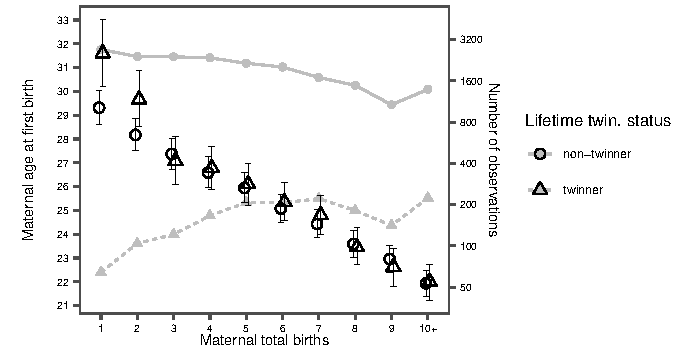
\includegraphics[height = 6cm]{../figures/figS1.pdf}
\end{center}
\caption{Relationship between lifetime twinning status, maternal total births and the age at first birth. The age at first birth was significantly higher for twinners with one ($\textrm{AFB}_\textrm{twinners}$ = 31.6 years; 95\% CI: 30.2, 33.0; $\textrm{AFB}_\textrm{non-twinners}$ = 29.3 years; 95\% CI 28.6, 30.0; delay for twinners = 27.5 months; 95\% CI: 11.9, 43.7) or two maternal total births ($\textrm{AFB}_\textrm{twinners}$ = 29.7 years; 95\% CI: 28.6, 30.8; $\textrm{AFB}_\textrm{non-twinners}$ = 28.2 years; 95\% CI: 27.5, 28.8; delay for twinners = 17.9 months; 95\% CI: 6.55, 29.4). Marginal predictions for the age at first reproduction are shown in black with open symbols. Their values are provided by the left y-axis. The distribution of maternal total births for both twinners and non-twinners is shown by the grey lines with filled symbols, with the numerical value given by the log-scaled y-axis on the right of the figure. 95\% CIs are based on 1000 bootstrap replicates for each depicted category of maternal total births.}
\end{figure}

\begin{figure}[H]
\begin{center}
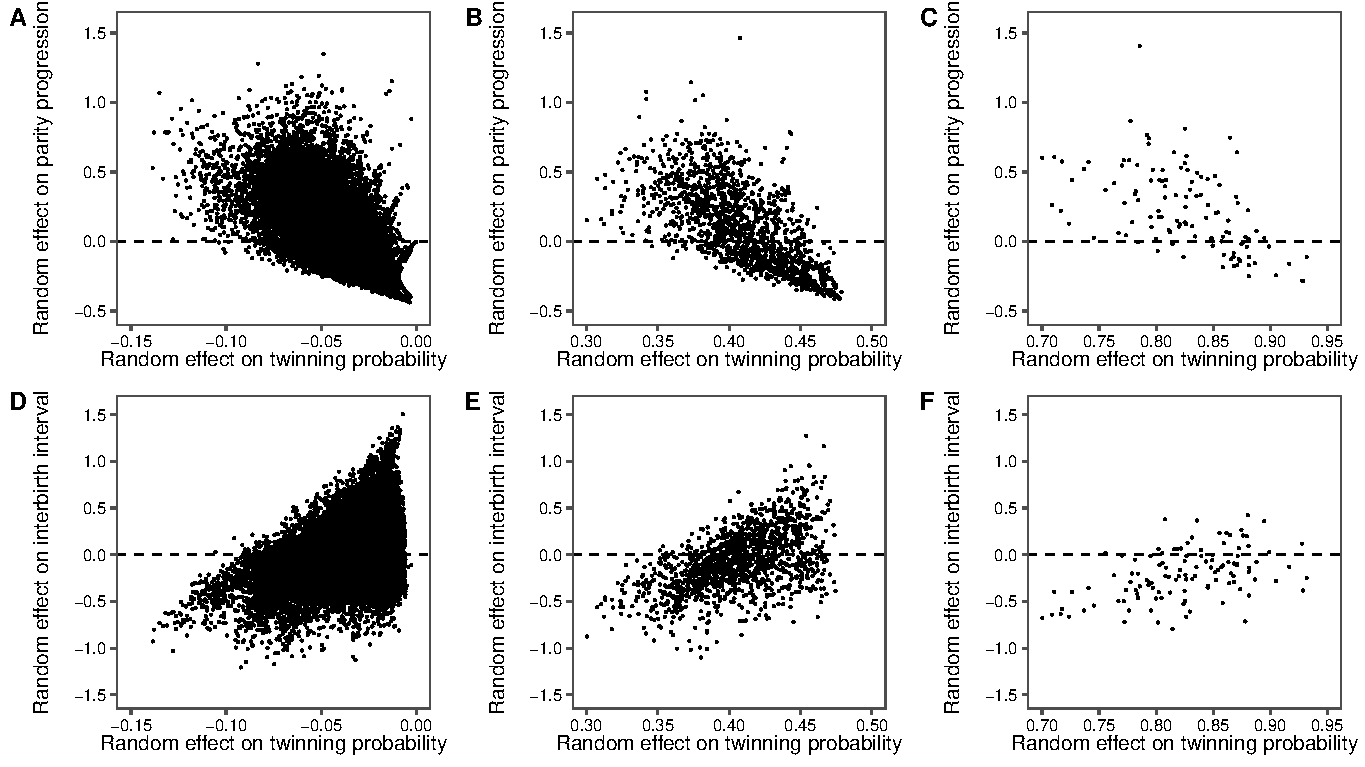
\includegraphics[height = 8cm]{../figures/figS2.pdf}
\end{center}
\caption{Relationships between the random effects for the three life history traits.
Top row (A-C) shows the relationship between the random effect from the fit of model 4 (the full model predicting parity progression; see Methods) and 6 (the full model predicting per-birth twinning probability). Bottom row (D-F) shows the relationship between the random effect from the fit of model 5 (the full model predicting the interbirth interval) and 6. Left column (A \& D) shows the relationship for mothers that did not produce any twins during their life. Middle column (B \& E) shows the relationship for mothers that produced twins once during their life. Right column (C \& F) shows the relationship for mothers that produced twins twice during their life. All axes are represented on the scale of the linear predictor of the corresponding models. Relationships for mothers that produced twins more than twice during their life are not displayed but follow similar patterns.}
\end{figure}

\begin{figure}[H]
\begin{center}
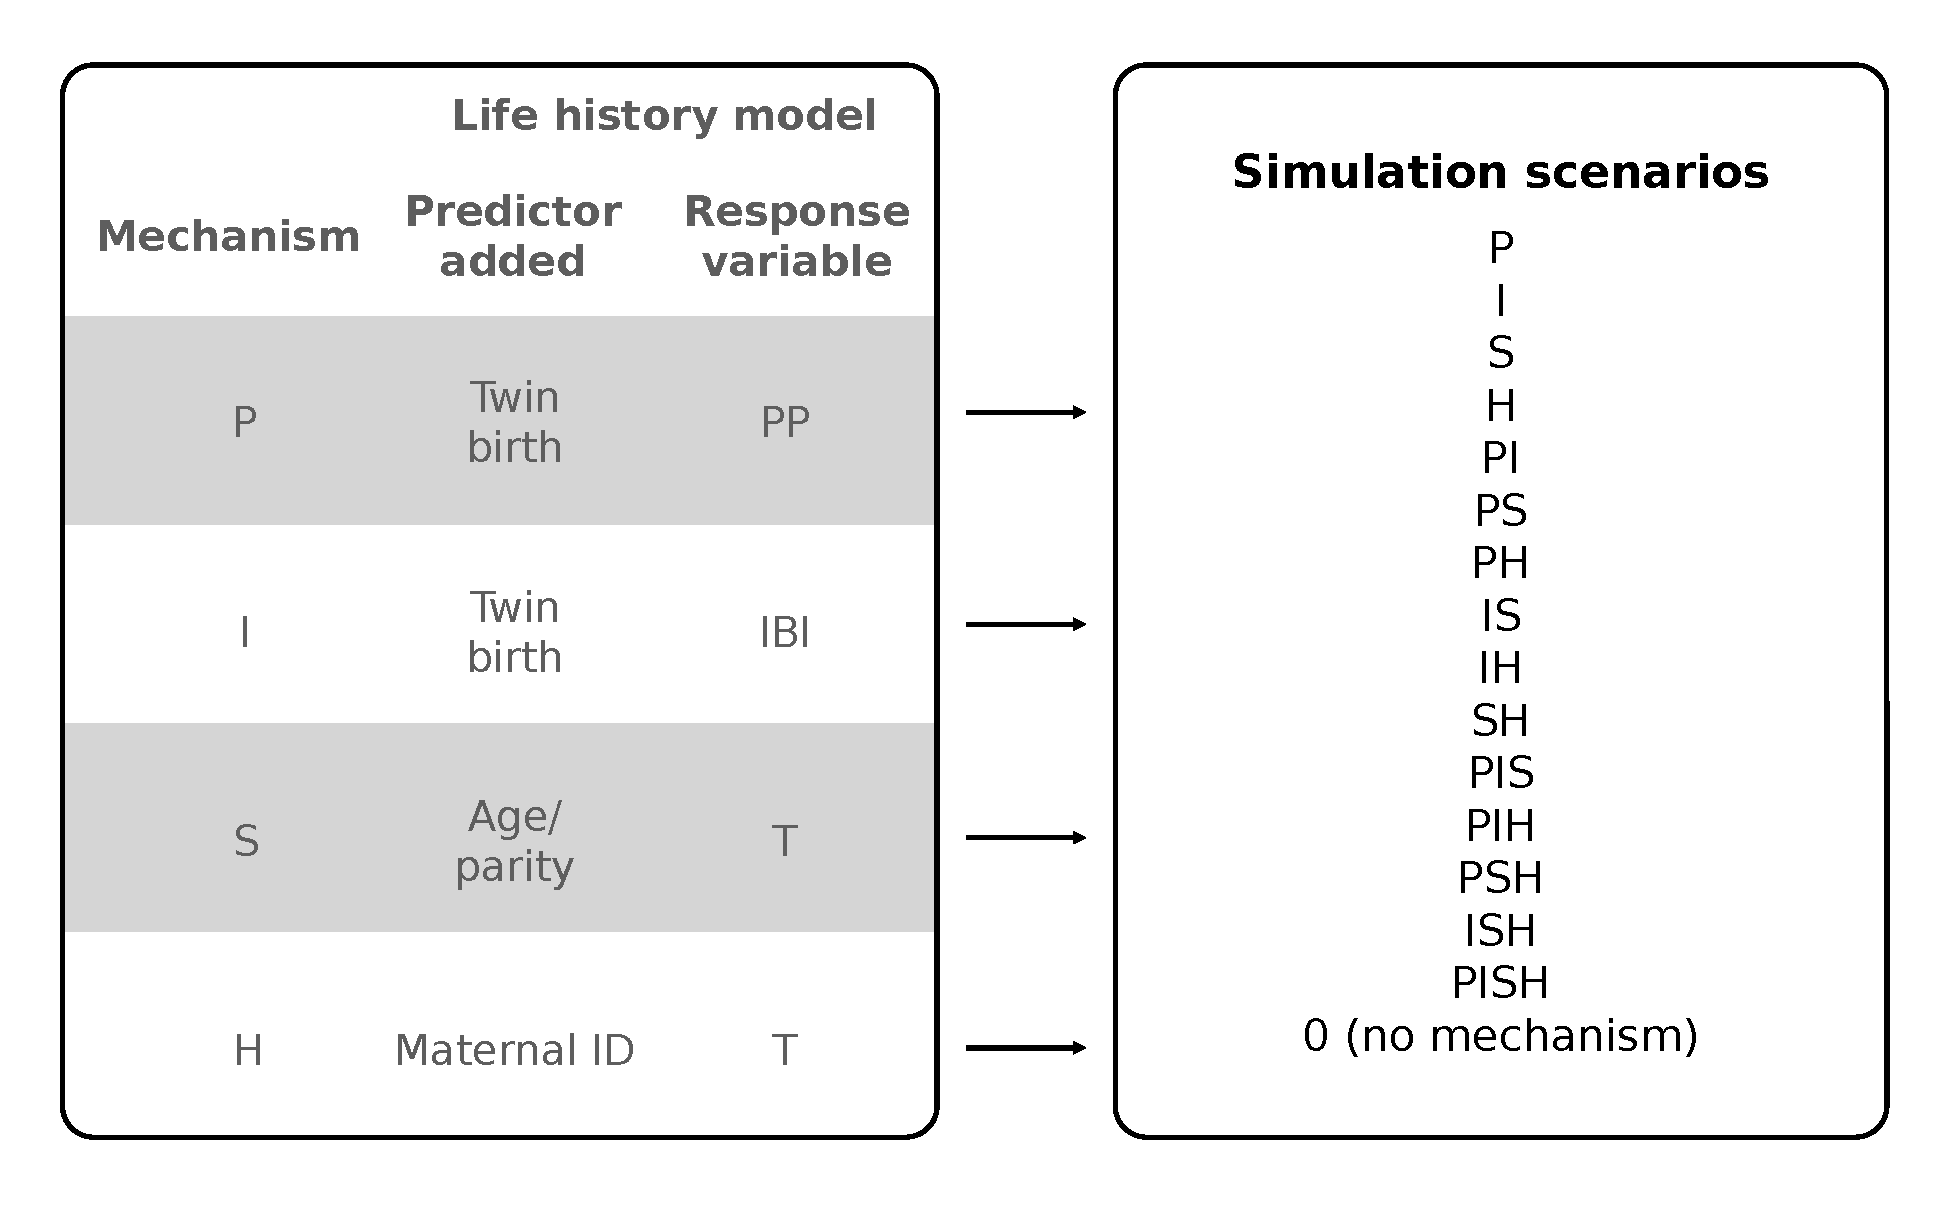
\includegraphics[height = 6cm]{../figures/figS3.pdf}
\end{center}
\caption{Hypothetical mechanisms tested by the simulation of alternative scenarios built around models predicting three life history events: parity progression (PP), interbirth interval (IBI) and twinning status of a given birth (T). The bubble on the left shows how the three life history models that were included in all simulation scenarios were modified to test each of the four hypothetical mechanisms (P, I, S, H; see section Results in main text for description). Each life history model describes the effect of predictors on a particular life history event. By default, each life history model includes an intercept and a random effect referring to the population. All models for PP and IBI also consider the effect of age/parity and maternal ID (see Methods). The bubble on the right shows the comprehensive set of combinations of the four mechanisms that were tested to produce simulation scenarios.}
\end{figure}

\begin{figure}[H]
\begin{center}
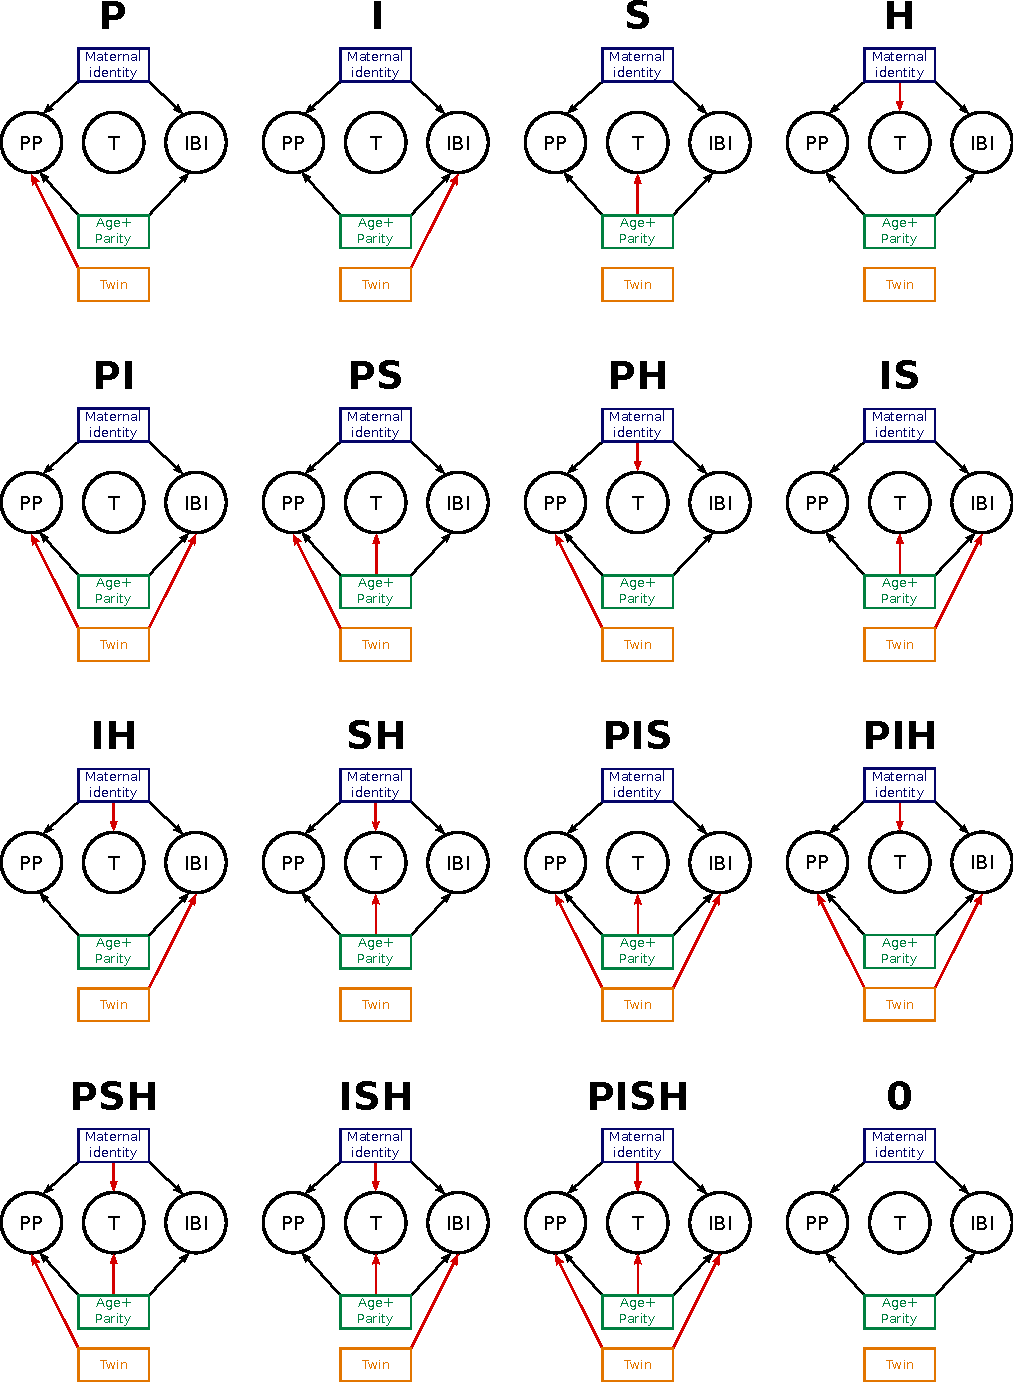
\includegraphics[width = 0.9\linewidth]{../figures/figS4.pdf}
\end{center}
\caption{Representation of the four mechanisms (row 1) used as the basis for 16 simulation scenarios evaluated (all rows). Circles represent the three life history events we considered: parity progression (PP), probability of twinning (T) and interbirth interval (IBI). The rectangles represent the variables potentially shaping these life history events — maternal age and parity at a given birth (referred to as Age + Parity above; and as $\mathtt{poly(cbind(age, parity), best\_order)}$ in model formulas) and whether the last birth was a twin birth or not (Twin above; $\mathtt{twin}$ in model formulas) — as well as a random effect capturing other sources of heterogeneity between mothers (Mum ID above; $\mathtt{maternal\_id}$ in model formulas). Black arrows represent relationships assumed in all simulation scenarios. Red arrows represent relationships \emph{activated} in order to investigate the role of each mechanism in accounting for the negative relationship between per-birth twinning probability and maternal total births.}
\end{figure}

\begin{figure}[H]
\begin{center}
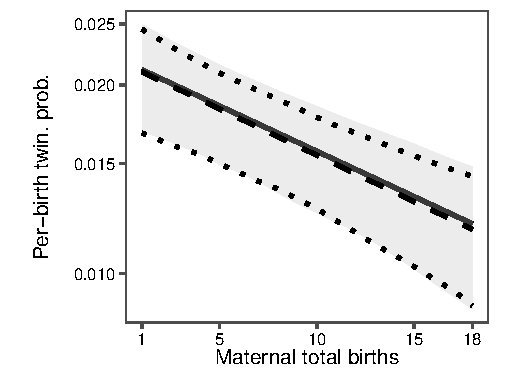
\includegraphics[height = 6cm]{../figures/figS5.pdf}
\end{center}
\caption{Relationship between the per-birth twinning probability and maternal total births. This figure reproduces the relationship shown in Main Text Fig. 2 (solid line) but additionally plots the relationship with the inclusion of data from families with missing birth month information (including the entire Norway dataset). This latter relationship is illustrated by the dashed regression line with an estimated slope $\beta'$ of -0.0346 (95\% CI: -0.0511, -0.0183), as well as with the dotted lines showing the location of the 95\% CI.}
\end{figure}

\begin{figure}[H]
\begin{center}
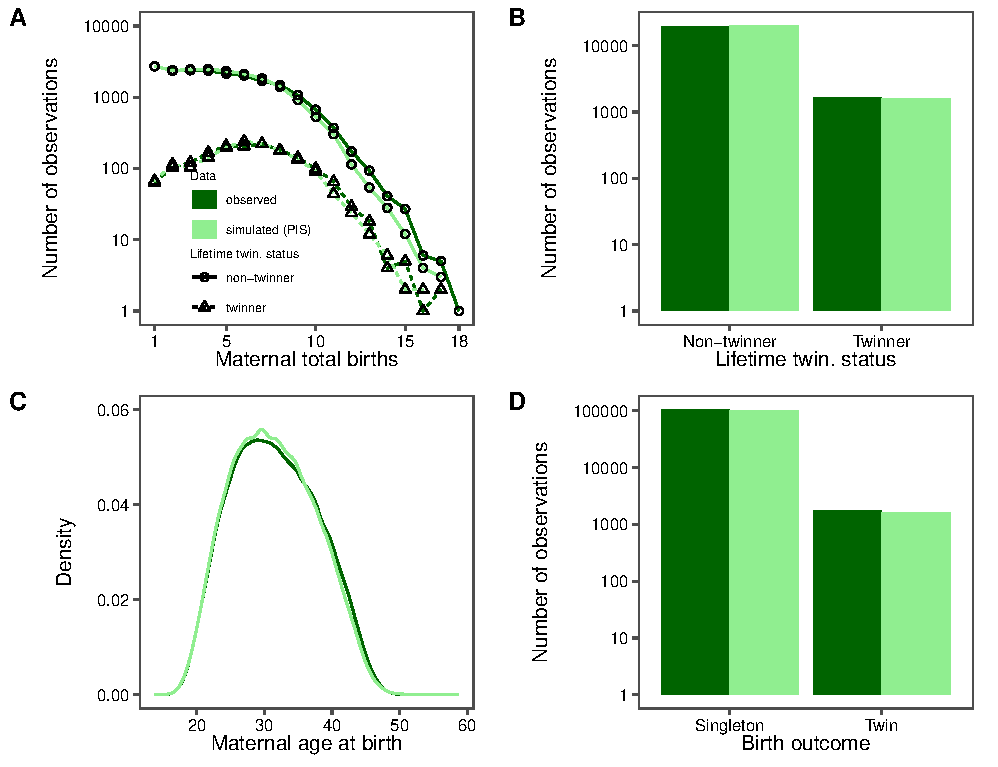
\includegraphics[height = 10cm]{../figures/figS6.pdf}
\end{center}
\caption{Comparison of different metrics between the real data and a dataset simulated under scenario PIS. A: distribution of maternal total births; B: number of twinners and non-twinners; C: distribution of maternal age at birth; D: number of singleton and twin births. The first row (A \& B) represents metrics computed at the level of mothers. The second row (C \& D) represents metrics computed at the level of births. All these plots show that the simulation scenario PIS produced fertility and twinning data similar to those measured on the observed data.}
\end{figure}

\begin{figure}[H]
\begin{center}
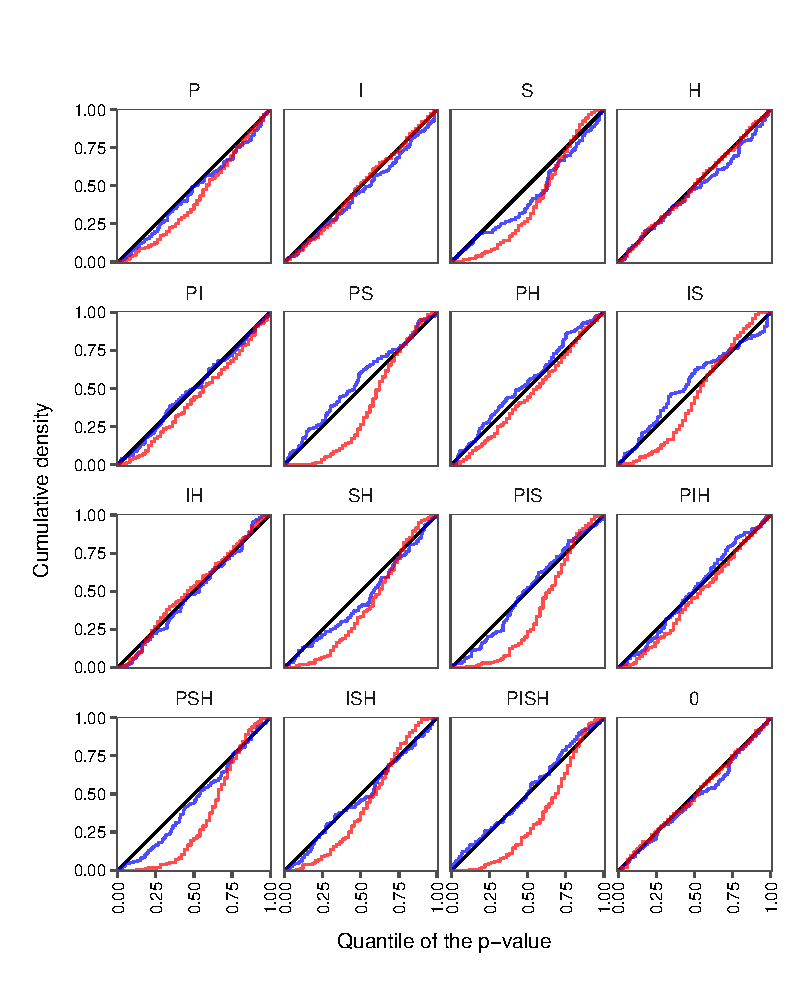
\includegraphics[width = 0.9\linewidth]{../figures/figS7.pdf}
\end{center}
\caption{Evaluation of the validity of the goodness-of-fit testing procedure. Each plot shows the empirical cumulative distribution of p-values for each tested simulation scenario, when the data were simulated under the same scenario. The goodness-of-fit test in such a case corresponds to the test of the null hypothesis when the null hypothesis is true. Therefore, the probability density of p-values should be uniform and the cumulative distribution should appear as the straight diagonal line depicted on the plots. However, the empirical cumulative distribution of p-values for the single-level bootstrap (shown in red) clearly departs from this expectation for scenarios including mechanisms P or S, showing that a correction is required. The empirical distributions of the double-bootstrap procedure (shown in blue) corrects this and show that the latter procedure can be applied for all scenarios.}
\end{figure}

\begin{table}[H]

\caption{\label{tab:tab1}Summary of the fit of model 1. The model fit corresponds to the fit of a model with the following formula: {\small$\mathtt{births\_total \sim 1 + twinner + (1 | pop)}$}. In all tables showing the summary of fits, values given in column 3 for fixed effects, random effects (if applicable) and the parameters of the response family (if applicable) are estimates. Other values are the results of computations.}
\centering
\fontsize{8}{10}\selectfont
\begin{tabular}[t]{>{\raggedright\arraybackslash}p{3cm}>{\raggedright\arraybackslash}p{5cm}rrr}
\toprule
Type & Variable & Value & Cond. SE & t-value\\
\midrule
\cellcolor{gray!6}{fixed effects} & \cellcolor{gray!6}{$\beta_1$} & \cellcolor{gray!6}{1.54} & \cellcolor{gray!6}{0.0319} & \cellcolor{gray!6}{48.1}\\
\cellcolor{gray!6}{} & \cellcolor{gray!6}{$\beta_{\mathtt{twinner}}$} & \cellcolor{gray!6}{0.279} & \cellcolor{gray!6}{0.0162} & \cellcolor{gray!6}{17.3}\\
random effects & variance between $\mathtt{pop}$ & 0.00785 &  & \\
\cellcolor{gray!6}{response family} & \cellcolor{gray!6}{truncated negative binomial with log link} & \cellcolor{gray!6}{} & \cellcolor{gray!6}{} & \cellcolor{gray!6}{}\\
\cellcolor{gray!6}{} & \cellcolor{gray!6}{shape parameter} & \cellcolor{gray!6}{4.73} & \cellcolor{gray!6}{} & \cellcolor{gray!6}{}\\
fit info & number of model parameters & 4 &  & \\
 & marginal log Likelihood & -50929 &  & \\
 & marginal AIC & 101866 &  & \\
 & conditional AIC (cAIC) & 101841 &  & \\
\cellcolor{gray!6}{data info} & \cellcolor{gray!6}{number of fitted observations (\emph{N})} & \cellcolor{gray!6}{21290} & \cellcolor{gray!6}{} & \cellcolor{gray!6}{}\\
\bottomrule
\end{tabular}
\end{table}


\begin{table}[H]

\caption{\label{tab:tab2}Summary of the fit of model 2. The model fit corresponds to the fit of a model with the following formula: {\small$\mathtt{twinner \sim 1 + births\_total + (1 | pop)}$}. See legend of Table S1 for more details.}
\centering
\fontsize{8}{10}\selectfont
\begin{tabular}[t]{>{\raggedright\arraybackslash}p{3cm}>{\raggedright\arraybackslash}p{5cm}rrr}
\toprule
Type & Variable & Value & Cond. SE & t-value\\
\midrule
\cellcolor{gray!6}{fixed effects} & \cellcolor{gray!6}{$\beta_1$} & \cellcolor{gray!6}{-3.35} & \cellcolor{gray!6}{0.112} & \cellcolor{gray!6}{-30}\\
\cellcolor{gray!6}{} & \cellcolor{gray!6}{$\beta_{\mathtt{births\_total}}$} & \cellcolor{gray!6}{0.162} & \cellcolor{gray!6}{0.00855} & \cellcolor{gray!6}{18.9}\\
random effects & variance between $\mathtt{pop}$ & 0.0697 &  & \\
\cellcolor{gray!6}{response family} & \cellcolor{gray!6}{binomial with logit link} & \cellcolor{gray!6}{} & \cellcolor{gray!6}{} & \cellcolor{gray!6}{}\\
fit info & number of model parameters & 3 &  & \\
 & marginal log Likelihood & -5548 &  & \\
 & marginal AIC & 11102 &  & \\
 & conditional AIC (cAIC) & 11086 &  & \\
\cellcolor{gray!6}{data info} & \cellcolor{gray!6}{number of fitted observations (\emph{N})} & \cellcolor{gray!6}{21290} & \cellcolor{gray!6}{} & \cellcolor{gray!6}{}\\
\bottomrule
\end{tabular}
\end{table}


\begin{table}

\caption{\label{tab:tab3}Summary of the fit of model 3. The model fit corresponds to the fit of a model with the following formula: {\small$\mathtt{cbind(twin\_total, singleton\_total) \sim 1 + births\_total + (1 | pop)}$}. See legend of Table S1 for more details.}
\centering
\fontsize{8}{10}\selectfont
\begin{tabular}[t]{>{\raggedright\arraybackslash}p{3cm}>{\raggedright\arraybackslash}p{5cm}rrr}
\toprule
Type & Variable & Value & Cond. SE & t-value\\
\midrule
\cellcolor{gray!6}{fixed effects} & \cellcolor{gray!6}{$\beta_1$} & \cellcolor{gray!6}{-3.83} & \cellcolor{gray!6}{0.104} & \cellcolor{gray!6}{-36.7}\\
\cellcolor{gray!6}{} & \cellcolor{gray!6}{$\beta_{\mathtt{births\_total}}$} & \cellcolor{gray!6}{-0.0338} & \cellcolor{gray!6}{0.00864} & \cellcolor{gray!6}{-3.92}\\
random effects & variance between $\mathtt{pop}$ & 0.0556 &  & \\
\cellcolor{gray!6}{response family} & \cellcolor{gray!6}{binomial with logit link} & \cellcolor{gray!6}{} & \cellcolor{gray!6}{} & \cellcolor{gray!6}{}\\
fit info & number of model parameters & 3 &  & \\
 & marginal log Likelihood & -5993 &  & \\
 & marginal AIC & 11992 &  & \\
 & conditional AIC (cAIC) & 11976 &  & \\
\cellcolor{gray!6}{data info} & \cellcolor{gray!6}{number of fitted observations (\emph{N})} & \cellcolor{gray!6}{21290} & \cellcolor{gray!6}{} & \cellcolor{gray!6}{}\\
\bottomrule
\end{tabular}
\end{table}


\begin{table}[H]

\caption{\label{tab:tab4}Summary of the fit of model 4. The model fit corresponds to the fit of a model with the following formula: {\small$\mathtt{PP \sim 1 + twin + poly(cbind(age, parity), 5) + (1 | maternal\_id) + (1 | pop)}$}. See legend of Supplementary Table 1 for more details.}
\centering
\fontsize{8}{10}\selectfont
\begin{tabular}[t]{>{\raggedright\arraybackslash}p{3cm}>{\raggedright\arraybackslash}p{5cm}rrr}
\toprule
Type & Variable & Value & Cond. SE & t-value\\
\midrule
\cellcolor{gray!6}{fixed effects} & \cellcolor{gray!6}{$\beta_1$} & \cellcolor{gray!6}{1.57} & \cellcolor{gray!6}{0.179} & \cellcolor{gray!6}{8.74}\\
\cellcolor{gray!6}{} & \cellcolor{gray!6}{$\beta_{\mathtt{twin}}$} & \cellcolor{gray!6}{-0.412} & \cellcolor{gray!6}{0.0636} & \cellcolor{gray!6}{-6.47}\\
\cellcolor{gray!6}{} & \cellcolor{gray!6}{$\beta_{\mathtt{age}}$} & \cellcolor{gray!6}{-420} & \cellcolor{gray!6}{59.7} & \cellcolor{gray!6}{-7.04}\\
\cellcolor{gray!6}{} & \cellcolor{gray!6}{$\beta_{\mathtt{age}^2}$} & \cellcolor{gray!6}{-185} & \cellcolor{gray!6}{51.7} & \cellcolor{gray!6}{-3.57}\\
\cellcolor{gray!6}{} & \cellcolor{gray!6}{$\beta_{\mathtt{age}^3}$} & \cellcolor{gray!6}{-43.7} & \cellcolor{gray!6}{32.6} & \cellcolor{gray!6}{-1.34}\\
\cellcolor{gray!6}{} & \cellcolor{gray!6}{$\beta_{\mathtt{age}^4}$} & \cellcolor{gray!6}{-15.7} & \cellcolor{gray!6}{14.3} & \cellcolor{gray!6}{-1.09}\\
\cellcolor{gray!6}{} & \cellcolor{gray!6}{$\beta_{\mathtt{age}^5}$} & \cellcolor{gray!6}{2.47} & \cellcolor{gray!6}{9.7} & \cellcolor{gray!6}{0.255}\\
\cellcolor{gray!6}{} & \cellcolor{gray!6}{$\beta_{\mathtt{parity}}$} & \cellcolor{gray!6}{49.1} & \cellcolor{gray!6}{97.6} & \cellcolor{gray!6}{0.502}\\
\cellcolor{gray!6}{} & \cellcolor{gray!6}{$\beta_{\mathtt{age}\times\mathtt{parity}}$} & \cellcolor{gray!6}{12922} & \cellcolor{gray!6}{39528} & \cellcolor{gray!6}{0.327}\\
\cellcolor{gray!6}{} & \cellcolor{gray!6}{$\beta_{\mathtt{age}^2\times\mathtt{parity}}$} & \cellcolor{gray!6}{-33721} & \cellcolor{gray!6}{30550} & \cellcolor{gray!6}{-1.1}\\
\cellcolor{gray!6}{} & \cellcolor{gray!6}{$\beta_{\mathtt{age}^3\times\mathtt{parity}}$} & \cellcolor{gray!6}{-395} & \cellcolor{gray!6}{14752} & \cellcolor{gray!6}{-0.0268}\\
\cellcolor{gray!6}{} & \cellcolor{gray!6}{$\beta_{\mathtt{age}^4\times\mathtt{parity}}$} & \cellcolor{gray!6}{-3270} & \cellcolor{gray!6}{6413} & \cellcolor{gray!6}{-0.51}\\
\cellcolor{gray!6}{} & \cellcolor{gray!6}{$\beta_{\mathtt{parity}^2}$} & \cellcolor{gray!6}{-18.3} & \cellcolor{gray!6}{105} & \cellcolor{gray!6}{-0.175}\\
\cellcolor{gray!6}{} & \cellcolor{gray!6}{$\beta_{\mathtt{age}\times\mathtt{parity}^2}$} & \cellcolor{gray!6}{23609} & \cellcolor{gray!6}{38306} & \cellcolor{gray!6}{0.616}\\
\cellcolor{gray!6}{} & \cellcolor{gray!6}{$\beta_{\mathtt{age}^2\times\mathtt{parity}^2}$} & \cellcolor{gray!6}{-5967} & \cellcolor{gray!6}{22834} & \cellcolor{gray!6}{-0.261}\\
\cellcolor{gray!6}{} & \cellcolor{gray!6}{$\beta_{\mathtt{age}^3\times\mathtt{parity}^2}$} & \cellcolor{gray!6}{10602} & \cellcolor{gray!6}{8890} & \cellcolor{gray!6}{1.19}\\
\cellcolor{gray!6}{} & \cellcolor{gray!6}{$\beta_{\mathtt{parity}^3}$} & \cellcolor{gray!6}{27} & \cellcolor{gray!6}{64.7} & \cellcolor{gray!6}{0.417}\\
\cellcolor{gray!6}{} & \cellcolor{gray!6}{$\beta_{\mathtt{age}\times\mathtt{parity}^3}$} & \cellcolor{gray!6}{-15417} & \cellcolor{gray!6}{19086} & \cellcolor{gray!6}{-0.808}\\
\cellcolor{gray!6}{} & \cellcolor{gray!6}{$\beta_{\mathtt{age}^2\times\mathtt{parity}^3}$} & \cellcolor{gray!6}{1259} & \cellcolor{gray!6}{8611} & \cellcolor{gray!6}{0.146}\\
\cellcolor{gray!6}{} & \cellcolor{gray!6}{$\beta_{\mathtt{parity}^4}$} & \cellcolor{gray!6}{24.5} & \cellcolor{gray!6}{21.4} & \cellcolor{gray!6}{1.14}\\
\cellcolor{gray!6}{} & \cellcolor{gray!6}{$\beta_{\mathtt{age}\times\mathtt{parity}^4}$} & \cellcolor{gray!6}{-1816} & \cellcolor{gray!6}{5027} & \cellcolor{gray!6}{-0.361}\\
\cellcolor{gray!6}{} & \cellcolor{gray!6}{$\beta_{\mathtt{parity}^5}$} & \cellcolor{gray!6}{-4.69} & \cellcolor{gray!6}{4.84} & \cellcolor{gray!6}{-0.97}\\
random effects & variance between $\mathtt{maternal\_id}$ & 0.465 &  & \\
 & variance between $\mathtt{pop}$ & 0.104 &  & \\
\cellcolor{gray!6}{response family} & \cellcolor{gray!6}{binomial with logit link} & \cellcolor{gray!6}{} & \cellcolor{gray!6}{} & \cellcolor{gray!6}{}\\
fit info & number of model parameters & 24 &  & \\
 & marginal log Likelihood & -40429 &  & \\
 & marginal AIC & 80905 &  & \\
 & conditional AIC (cAIC) & 80276 &  & \\
\cellcolor{gray!6}{data info} & \cellcolor{gray!6}{number of fitted observations (\emph{N})} & \cellcolor{gray!6}{105833} & \cellcolor{gray!6}{} & \cellcolor{gray!6}{}\\
\bottomrule
\end{tabular}
\end{table}


\begin{table}[H]

\caption{\label{tab:tab5}Summary of the fit of model 5. The model fit corresponds to the fit of a model with the following formula: {\small$\mathtt{IBI \sim 1 + twin + poly(cbind(age, parity), 6) + (1 | maternal\_id) + (1 | pop)}$}. Note that the variable \texttt{IBI} fitted in the model actually corresponds to the duration of interbirth interval minus six months. This rescaling prevents numerical issues during the simulations. When this fitted model is used for predictions (in plots or to compute effect sizes), the missing six months are reintroduced to produce correct results. See legend of Table S1 for other details.}
\centering
\fontsize{8}{10}\selectfont
\begin{tabular}[t]{>{\raggedright\arraybackslash}p{3cm}>{\raggedright\arraybackslash}p{5cm}rrr}
\toprule
Type & Variable & Value & Cond. SE & t-value\\
\midrule
\cellcolor{gray!6}{fixed effects} & \cellcolor{gray!6}{$\beta_1$} & \cellcolor{gray!6}{3.44} & \cellcolor{gray!6}{0.0579} & \cellcolor{gray!6}{59.5}\\
\cellcolor{gray!6}{} & \cellcolor{gray!6}{$\beta_{\mathtt{twin}}$} & \cellcolor{gray!6}{-0.0328} & \cellcolor{gray!6}{0.015} & \cellcolor{gray!6}{-2.18}\\
\cellcolor{gray!6}{} & \cellcolor{gray!6}{$\beta_{\mathtt{age}}$} & \cellcolor{gray!6}{-63.6} & \cellcolor{gray!6}{21.9} & \cellcolor{gray!6}{-2.9}\\
\cellcolor{gray!6}{} & \cellcolor{gray!6}{$\beta_{\mathtt{age}^2}$} & \cellcolor{gray!6}{39.7} & \cellcolor{gray!6}{19.6} & \cellcolor{gray!6}{2.02}\\
\cellcolor{gray!6}{} & \cellcolor{gray!6}{$\beta_{\mathtt{age}^3}$} & \cellcolor{gray!6}{-31.3} & \cellcolor{gray!6}{13} & \cellcolor{gray!6}{-2.41}\\
\cellcolor{gray!6}{} & \cellcolor{gray!6}{$\beta_{\mathtt{age}^4}$} & \cellcolor{gray!6}{15} & \cellcolor{gray!6}{6.31} & \cellcolor{gray!6}{2.38}\\
\cellcolor{gray!6}{} & \cellcolor{gray!6}{$\beta_{\mathtt{age}^5}$} & \cellcolor{gray!6}{-5} & \cellcolor{gray!6}{2.42} & \cellcolor{gray!6}{-2.07}\\
\cellcolor{gray!6}{} & \cellcolor{gray!6}{$\beta_{\mathtt{age}^6}$} & \cellcolor{gray!6}{4.01} & \cellcolor{gray!6}{1.01} & \cellcolor{gray!6}{3.95}\\
\cellcolor{gray!6}{} & \cellcolor{gray!6}{$\beta_{\mathtt{parity}}$} & \cellcolor{gray!6}{121} & \cellcolor{gray!6}{40.7} & \cellcolor{gray!6}{2.96}\\
\cellcolor{gray!6}{} & \cellcolor{gray!6}{$\beta_{\mathtt{age}\times\mathtt{parity}}$} & \cellcolor{gray!6}{-29804} & \cellcolor{gray!6}{15604} & \cellcolor{gray!6}{-1.91}\\
\cellcolor{gray!6}{} & \cellcolor{gray!6}{$\beta_{\mathtt{age}^2\times\mathtt{parity}}$} & \cellcolor{gray!6}{26630} & \cellcolor{gray!6}{12833} & \cellcolor{gray!6}{2.08}\\
\cellcolor{gray!6}{} & \cellcolor{gray!6}{$\beta_{\mathtt{age}^3\times\mathtt{parity}}$} & \cellcolor{gray!6}{-15687} & \cellcolor{gray!6}{7263} & \cellcolor{gray!6}{-2.16}\\
\cellcolor{gray!6}{} & \cellcolor{gray!6}{$\beta_{\mathtt{age}^4\times\mathtt{parity}}$} & \cellcolor{gray!6}{5901} & \cellcolor{gray!6}{2912} & \cellcolor{gray!6}{2.03}\\
\cellcolor{gray!6}{} & \cellcolor{gray!6}{$\beta_{\mathtt{age}^5\times\mathtt{parity}}$} & \cellcolor{gray!6}{-2056} & \cellcolor{gray!6}{883} & \cellcolor{gray!6}{-2.33}\\
\cellcolor{gray!6}{} & \cellcolor{gray!6}{$\beta_{\mathtt{parity}^2}$} & \cellcolor{gray!6}{75.7} & \cellcolor{gray!6}{54.5} & \cellcolor{gray!6}{1.39}\\
\cellcolor{gray!6}{} & \cellcolor{gray!6}{$\beta_{\mathtt{age}\times\mathtt{parity}^2}$} & \cellcolor{gray!6}{-30418} & \cellcolor{gray!6}{19139} & \cellcolor{gray!6}{-1.59}\\
\cellcolor{gray!6}{} & \cellcolor{gray!6}{$\beta_{\mathtt{age}^2\times\mathtt{parity}^2}$} & \cellcolor{gray!6}{24308} & \cellcolor{gray!6}{13414} & \cellcolor{gray!6}{1.81}\\
\cellcolor{gray!6}{} & \cellcolor{gray!6}{$\beta_{\mathtt{age}^3\times\mathtt{parity}^2}$} & \cellcolor{gray!6}{-11197} & \cellcolor{gray!6}{5960} & \cellcolor{gray!6}{-1.88}\\
\cellcolor{gray!6}{} & \cellcolor{gray!6}{$\beta_{\mathtt{age}^4\times\mathtt{parity}^2}$} & \cellcolor{gray!6}{3100} & \cellcolor{gray!6}{1618} & \cellcolor{gray!6}{1.92}\\
\cellcolor{gray!6}{} & \cellcolor{gray!6}{$\beta_{\mathtt{parity}^3}$} & \cellcolor{gray!6}{53} & \cellcolor{gray!6}{42.1} & \cellcolor{gray!6}{1.26}\\
\cellcolor{gray!6}{} & \cellcolor{gray!6}{$\beta_{\mathtt{age}\times\mathtt{parity}^3}$} & \cellcolor{gray!6}{-17528} & \cellcolor{gray!6}{12996} & \cellcolor{gray!6}{-1.35}\\
\cellcolor{gray!6}{} & \cellcolor{gray!6}{$\beta_{\mathtt{age}^2\times\mathtt{parity}^3}$} & \cellcolor{gray!6}{9735} & \cellcolor{gray!6}{7207} & \cellcolor{gray!6}{1.35}\\
\cellcolor{gray!6}{} & \cellcolor{gray!6}{$\beta_{\mathtt{age}^3\times\mathtt{parity}^3}$} & \cellcolor{gray!6}{-2955} & \cellcolor{gray!6}{2067} & \cellcolor{gray!6}{-1.43}\\
\cellcolor{gray!6}{} & \cellcolor{gray!6}{$\beta_{\mathtt{parity}^4}$} & \cellcolor{gray!6}{19} & \cellcolor{gray!6}{19} & \cellcolor{gray!6}{1}\\
\cellcolor{gray!6}{} & \cellcolor{gray!6}{$\beta_{\mathtt{age}\times\mathtt{parity}^4}$} & \cellcolor{gray!6}{-4658} & \cellcolor{gray!6}{4824} & \cellcolor{gray!6}{-0.966}\\
\cellcolor{gray!6}{} & \cellcolor{gray!6}{$\beta_{\mathtt{age}^2\times\mathtt{parity}^4}$} & \cellcolor{gray!6}{1902} & \cellcolor{gray!6}{1773} & \cellcolor{gray!6}{1.07}\\
\cellcolor{gray!6}{} & \cellcolor{gray!6}{$\beta_{\mathtt{parity}^5}$} & \cellcolor{gray!6}{7.84} & \cellcolor{gray!6}{5.26} & \cellcolor{gray!6}{1.49}\\
\cellcolor{gray!6}{} & \cellcolor{gray!6}{$\beta_{\mathtt{age}\times\mathtt{parity}^5}$} & \cellcolor{gray!6}{-1418} & \cellcolor{gray!6}{970} & \cellcolor{gray!6}{-1.46}\\
\cellcolor{gray!6}{} & \cellcolor{gray!6}{$\beta_{\mathtt{parity}^6}$} & \cellcolor{gray!6}{1.68} & \cellcolor{gray!6}{1.04} & \cellcolor{gray!6}{1.61}\\
random effects & variance between $\mathtt{maternal\_id}$ & 0.163 &  & \\
 & variance between $\mathtt{pop}$ & 0.00375 &  & \\
\cellcolor{gray!6}{response family} & \cellcolor{gray!6}{negative binomial with log link} & \cellcolor{gray!6}{} & \cellcolor{gray!6}{} & \cellcolor{gray!6}{}\\
\cellcolor{gray!6}{} & \cellcolor{gray!6}{shape parameter} & \cellcolor{gray!6}{5.2} & \cellcolor{gray!6}{} & \cellcolor{gray!6}{}\\
fit info & number of model parameters & 32 &  & \\
 & marginal log Likelihood & -337275 &  & \\
 & marginal AIC & 674614 &  & \\
 & conditional AIC (cAIC) & 663067 &  & \\
\cellcolor{gray!6}{data info} & \cellcolor{gray!6}{number of fitted observations (\emph{N})} & \cellcolor{gray!6}{84543} & \cellcolor{gray!6}{} & \cellcolor{gray!6}{}\\
\bottomrule
\end{tabular}
\end{table}


\begin{table}[H]

\caption{\label{tab:tab6}Summary of the fit of model 6. The model fit corresponds to the fit of a model with the following formula: {\small$\mathtt{T \sim 1 + poly(cbind(age, parity), 3) + (1 | maternal\_id) + (1 | pop)}$}. See legend of Supplementary Table 1 for more details.}
\centering
\fontsize{8}{10}\selectfont
\begin{tabular}[t]{>{\raggedright\arraybackslash}p{3cm}>{\raggedright\arraybackslash}p{5cm}rrr}
\toprule
Type & Variable & Value & Cond. SE & t-value\\
\midrule
\cellcolor{gray!6}{fixed effects} & \cellcolor{gray!6}{$\beta_1$} & \cellcolor{gray!6}{-4.1} & \cellcolor{gray!6}{0.113} & \cellcolor{gray!6}{-36.4}\\
\cellcolor{gray!6}{} & \cellcolor{gray!6}{$\beta_{\mathtt{age}}$} & \cellcolor{gray!6}{73.7} & \cellcolor{gray!6}{31.1} & \cellcolor{gray!6}{2.37}\\
\cellcolor{gray!6}{} & \cellcolor{gray!6}{$\beta_{\mathtt{age}^2}$} & \cellcolor{gray!6}{-61.2} & \cellcolor{gray!6}{17.2} & \cellcolor{gray!6}{-3.55}\\
\cellcolor{gray!6}{} & \cellcolor{gray!6}{$\beta_{\mathtt{age}^3}$} & \cellcolor{gray!6}{-47.1} & \cellcolor{gray!6}{16.4} & \cellcolor{gray!6}{-2.87}\\
\cellcolor{gray!6}{} & \cellcolor{gray!6}{$\beta_{\mathtt{parity}}$} & \cellcolor{gray!6}{-0.936} & \cellcolor{gray!6}{40.1} & \cellcolor{gray!6}{-0.0233}\\
\cellcolor{gray!6}{} & \cellcolor{gray!6}{$\beta_{\mathtt{age}\times\mathtt{parity}}$} & \cellcolor{gray!6}{-4006} & \cellcolor{gray!6}{11890} & \cellcolor{gray!6}{-0.337}\\
\cellcolor{gray!6}{} & \cellcolor{gray!6}{$\beta_{\mathtt{age}^2\times\mathtt{parity}}$} & \cellcolor{gray!6}{7710} & \cellcolor{gray!6}{8669} & \cellcolor{gray!6}{0.889}\\
\cellcolor{gray!6}{} & \cellcolor{gray!6}{$\beta_{\mathtt{parity}^2}$} & \cellcolor{gray!6}{19} & \cellcolor{gray!6}{27.3} & \cellcolor{gray!6}{0.694}\\
\cellcolor{gray!6}{} & \cellcolor{gray!6}{$\beta_{\mathtt{age}\times\mathtt{parity}^2}$} & \cellcolor{gray!6}{-4380} & \cellcolor{gray!6}{8121} & \cellcolor{gray!6}{-0.539}\\
\cellcolor{gray!6}{} & \cellcolor{gray!6}{$\beta_{\mathtt{parity}^3}$} & \cellcolor{gray!6}{-18.6} & \cellcolor{gray!6}{14.1} & \cellcolor{gray!6}{-1.32}\\
random effects & variance between $\mathtt{maternal\_id}$ & 0.485 &  & \\
 & variance between $\mathtt{pop}$ & 0.0571 &  & \\
\cellcolor{gray!6}{response family} & \cellcolor{gray!6}{binomial with logit link} & \cellcolor{gray!6}{} & \cellcolor{gray!6}{} & \cellcolor{gray!6}{}\\
fit info & number of model parameters & 12 &  & \\
 & marginal log Likelihood & -8828 &  & \\
 & marginal AIC & 17681 &  & \\
 & conditional AIC (cAIC) & 17644 &  & \\
\cellcolor{gray!6}{data info} & \cellcolor{gray!6}{number of fitted observations (\emph{N})} & \cellcolor{gray!6}{105833} & \cellcolor{gray!6}{} & \cellcolor{gray!6}{}\\
\bottomrule
\end{tabular}
\end{table}


\begin{table}[H]

\caption{\label{tab:tab7}Summary of the fit of model 7. The model fit corresponds to the fit of a model with the following formula: {\small$\mathtt{AFB \sim 1 + twinner * births\_total\_fac + (1 | pop)}$}. See legend of Supplementary Table 1 for more details.}
\centering
\fontsize{8}{10}\selectfont
\begin{tabular}[t]{>{\raggedright\arraybackslash}p{3cm}>{\raggedright\arraybackslash}p{5cm}rrr}
\toprule
Type & Variable & Value & Cond. SE & t-value\\
\midrule
\cellcolor{gray!6}{fixed effects} & \cellcolor{gray!6}{$\beta_1$} & \cellcolor{gray!6}{5.86} & \cellcolor{gray!6}{0.0123} & \cellcolor{gray!6}{479}\\
\cellcolor{gray!6}{} & \cellcolor{gray!6}{$\beta_{\mathtt{twinner}}$} & \cellcolor{gray!6}{0.0752} & \cellcolor{gray!6}{0.0207} & \cellcolor{gray!6}{3.63}\\
\cellcolor{gray!6}{} & \cellcolor{gray!6}{$\beta_{\mathtt{births\_total\_fac2}}$} & \cellcolor{gray!6}{-0.0396} & \cellcolor{gray!6}{0.00461} & \cellcolor{gray!6}{-8.6}\\
\cellcolor{gray!6}{} & \cellcolor{gray!6}{$\beta_{\mathtt{births\_total\_fac3}}$} & \cellcolor{gray!6}{-0.0686} & \cellcolor{gray!6}{0.00462} & \cellcolor{gray!6}{-14.8}\\
\cellcolor{gray!6}{} & \cellcolor{gray!6}{$\beta_{\mathtt{births\_total\_fac4}}$} & \cellcolor{gray!6}{-0.0977} & \cellcolor{gray!6}{0.00465} & \cellcolor{gray!6}{-21}\\
\cellcolor{gray!6}{} & \cellcolor{gray!6}{$\beta_{\mathtt{births\_total\_fac5}}$} & \cellcolor{gray!6}{-0.122} & \cellcolor{gray!6}{0.00477} & \cellcolor{gray!6}{-25.6}\\
\cellcolor{gray!6}{} & \cellcolor{gray!6}{$\beta_{\mathtt{births\_total\_fac6}}$} & \cellcolor{gray!6}{-0.156} & \cellcolor{gray!6}{0.00486} & \cellcolor{gray!6}{-32.1}\\
\cellcolor{gray!6}{} & \cellcolor{gray!6}{$\beta_{\mathtt{births\_total\_fac7}}$} & \cellcolor{gray!6}{-0.182} & \cellcolor{gray!6}{0.00513} & \cellcolor{gray!6}{-35.5}\\
\cellcolor{gray!6}{} & \cellcolor{gray!6}{$\beta_{\mathtt{births\_total\_fac8}}$} & \cellcolor{gray!6}{-0.217} & \cellcolor{gray!6}{0.00536} & \cellcolor{gray!6}{-40.5}\\
\cellcolor{gray!6}{} & \cellcolor{gray!6}{$\beta_{\mathtt{births\_total\_fac9}}$} & \cellcolor{gray!6}{-0.244} & \cellcolor{gray!6}{0.00601} & \cellcolor{gray!6}{-40.7}\\
\cellcolor{gray!6}{} & \cellcolor{gray!6}{$\beta_{\mathtt{births\_total\_fac10+}}$} & \cellcolor{gray!6}{-0.29} & \cellcolor{gray!6}{0.00551} & \cellcolor{gray!6}{-52.6}\\
\cellcolor{gray!6}{} & \cellcolor{gray!6}{$\beta_{\mathtt{twinner:births\_total\_fac2}}$} & \cellcolor{gray!6}{-0.0236} & \cellcolor{gray!6}{0.0264} & \cellcolor{gray!6}{-0.894}\\
\cellcolor{gray!6}{} & \cellcolor{gray!6}{$\beta_{\mathtt{twinner:births\_total\_fac3}}$} & \cellcolor{gray!6}{-0.086} & \cellcolor{gray!6}{0.0258} & \cellcolor{gray!6}{-3.34}\\
\cellcolor{gray!6}{} & \cellcolor{gray!6}{$\beta_{\mathtt{twinner:births\_total\_fac4}}$} & \cellcolor{gray!6}{-0.0676} & \cellcolor{gray!6}{0.0246} & \cellcolor{gray!6}{-2.75}\\
\cellcolor{gray!6}{} & \cellcolor{gray!6}{$\beta_{\mathtt{twinner:births\_total\_fac5}}$} & \cellcolor{gray!6}{-0.0688} & \cellcolor{gray!6}{0.0239} & \cellcolor{gray!6}{-2.87}\\
\cellcolor{gray!6}{} & \cellcolor{gray!6}{$\beta_{\mathtt{twinner:births\_total\_fac6}}$} & \cellcolor{gray!6}{-0.0643} & \cellcolor{gray!6}{0.024} & \cellcolor{gray!6}{-2.68}\\
\cellcolor{gray!6}{} & \cellcolor{gray!6}{$\beta_{\mathtt{twinner:births\_total\_fac7}}$} & \cellcolor{gray!6}{-0.06} & \cellcolor{gray!6}{0.0239} & \cellcolor{gray!6}{-2.52}\\
\cellcolor{gray!6}{} & \cellcolor{gray!6}{$\beta_{\mathtt{twinner:births\_total\_fac8}}$} & \cellcolor{gray!6}{-0.081} & \cellcolor{gray!6}{0.0245} & \cellcolor{gray!6}{-3.31}\\
\cellcolor{gray!6}{} & \cellcolor{gray!6}{$\beta_{\mathtt{twinner:births\_total\_fac9}}$} & \cellcolor{gray!6}{-0.0893} & \cellcolor{gray!6}{0.0255} & \cellcolor{gray!6}{-3.5}\\
\cellcolor{gray!6}{} & \cellcolor{gray!6}{$\beta_{\mathtt{twinner:births\_total\_fac10+}}$} & \cellcolor{gray!6}{-0.0719} & \cellcolor{gray!6}{0.024} & \cellcolor{gray!6}{-3}\\
random effects & variance between $\mathtt{pop}$ & 0.00111 &  & \\
\cellcolor{gray!6}{response family} & \cellcolor{gray!6}{negative binomial with log link} & \cellcolor{gray!6}{} & \cellcolor{gray!6}{} & \cellcolor{gray!6}{}\\
\cellcolor{gray!6}{} & \cellcolor{gray!6}{shape parameter} & \cellcolor{gray!6}{41.5} & \cellcolor{gray!6}{} & \cellcolor{gray!6}{}\\
fit info & number of model parameters & 22 &  & \\
 & marginal log Likelihood & -113839 &  & \\
 & marginal AIC & 227722 &  & \\
 & conditional AIC (cAIC) & 227691 &  & \\
\cellcolor{gray!6}{data info} & \cellcolor{gray!6}{number of fitted observations (\emph{N})} & \cellcolor{gray!6}{21290} & \cellcolor{gray!6}{} & \cellcolor{gray!6}{}\\
\bottomrule
\end{tabular}
\end{table}


\begin{table}

\caption{\label{tab:tab8}Summary of the fit of model 8. The model fit corresponds to the fit of a model with the following formula: {\small$\mathtt{PP \sim 1 + poly(cbind(age, parity), 5) + (1 | maternal\_id) + (1 | pop)}$}. See legend of Table S1 for more details.}
\centering
\fontsize{8}{10}\selectfont
\begin{tabular}[t]{>{\raggedright\arraybackslash}p{3cm}>{\raggedright\arraybackslash}p{5cm}rrr}
\toprule
Type & Variable & Value & Cond. SE & t-value\\
\midrule
\cellcolor{gray!6}{fixed effects} & \cellcolor{gray!6}{$\beta_1$} & \cellcolor{gray!6}{1.56} & \cellcolor{gray!6}{0.179} & \cellcolor{gray!6}{8.67}\\
\cellcolor{gray!6}{} & \cellcolor{gray!6}{$\beta_{\mathtt{age}}$} & \cellcolor{gray!6}{-421} & \cellcolor{gray!6}{59.7} & \cellcolor{gray!6}{-7.04}\\
\cellcolor{gray!6}{} & \cellcolor{gray!6}{$\beta_{\mathtt{age}^2}$} & \cellcolor{gray!6}{-185} & \cellcolor{gray!6}{51.8} & \cellcolor{gray!6}{-3.57}\\
\cellcolor{gray!6}{} & \cellcolor{gray!6}{$\beta_{\mathtt{age}^3}$} & \cellcolor{gray!6}{-43.4} & \cellcolor{gray!6}{32.6} & \cellcolor{gray!6}{-1.33}\\
\cellcolor{gray!6}{} & \cellcolor{gray!6}{$\beta_{\mathtt{age}^4}$} & \cellcolor{gray!6}{-15.8} & \cellcolor{gray!6}{14.4} & \cellcolor{gray!6}{-1.1}\\
\cellcolor{gray!6}{} & \cellcolor{gray!6}{$\beta_{\mathtt{age}^5}$} & \cellcolor{gray!6}{2.3} & \cellcolor{gray!6}{9.7} & \cellcolor{gray!6}{0.237}\\
\cellcolor{gray!6}{} & \cellcolor{gray!6}{$\beta_{\mathtt{parity}}$} & \cellcolor{gray!6}{48} & \cellcolor{gray!6}{97.7} & \cellcolor{gray!6}{0.491}\\
\cellcolor{gray!6}{} & \cellcolor{gray!6}{$\beta_{\mathtt{age}\times\mathtt{parity}}$} & \cellcolor{gray!6}{13240} & \cellcolor{gray!6}{39545} & \cellcolor{gray!6}{0.335}\\
\cellcolor{gray!6}{} & \cellcolor{gray!6}{$\beta_{\mathtt{age}^2\times\mathtt{parity}}$} & \cellcolor{gray!6}{-34019} & \cellcolor{gray!6}{30565} & \cellcolor{gray!6}{-1.11}\\
\cellcolor{gray!6}{} & \cellcolor{gray!6}{$\beta_{\mathtt{age}^3\times\mathtt{parity}}$} & \cellcolor{gray!6}{-330} & \cellcolor{gray!6}{14760} & \cellcolor{gray!6}{-0.0224}\\
\cellcolor{gray!6}{} & \cellcolor{gray!6}{$\beta_{\mathtt{age}^4\times\mathtt{parity}}$} & \cellcolor{gray!6}{-3263} & \cellcolor{gray!6}{6416} & \cellcolor{gray!6}{-0.509}\\
\cellcolor{gray!6}{} & \cellcolor{gray!6}{$\beta_{\mathtt{parity}^2}$} & \cellcolor{gray!6}{-19.8} & \cellcolor{gray!6}{105} & \cellcolor{gray!6}{-0.188}\\
\cellcolor{gray!6}{} & \cellcolor{gray!6}{$\beta_{\mathtt{age}\times\mathtt{parity}^2}$} & \cellcolor{gray!6}{24157} & \cellcolor{gray!6}{38317} & \cellcolor{gray!6}{0.63}\\
\cellcolor{gray!6}{} & \cellcolor{gray!6}{$\beta_{\mathtt{age}^2\times\mathtt{parity}^2}$} & \cellcolor{gray!6}{-6236} & \cellcolor{gray!6}{22842} & \cellcolor{gray!6}{-0.273}\\
\cellcolor{gray!6}{} & \cellcolor{gray!6}{$\beta_{\mathtt{age}^3\times\mathtt{parity}^2}$} & \cellcolor{gray!6}{10729} & \cellcolor{gray!6}{8894} & \cellcolor{gray!6}{1.21}\\
\cellcolor{gray!6}{} & \cellcolor{gray!6}{$\beta_{\mathtt{parity}^3}$} & \cellcolor{gray!6}{25.9} & \cellcolor{gray!6}{64.7} & \cellcolor{gray!6}{0.4}\\
\cellcolor{gray!6}{} & \cellcolor{gray!6}{$\beta_{\mathtt{age}\times\mathtt{parity}^3}$} & \cellcolor{gray!6}{-15049} & \cellcolor{gray!6}{19092} & \cellcolor{gray!6}{-0.788}\\
\cellcolor{gray!6}{} & \cellcolor{gray!6}{$\beta_{\mathtt{age}^2\times\mathtt{parity}^3}$} & \cellcolor{gray!6}{1073} & \cellcolor{gray!6}{8613} & \cellcolor{gray!6}{0.125}\\
\cellcolor{gray!6}{} & \cellcolor{gray!6}{$\beta_{\mathtt{parity}^4}$} & \cellcolor{gray!6}{24} & \cellcolor{gray!6}{21.4} & \cellcolor{gray!6}{1.12}\\
\cellcolor{gray!6}{} & \cellcolor{gray!6}{$\beta_{\mathtt{age}\times\mathtt{parity}^4}$} & \cellcolor{gray!6}{-1749} & \cellcolor{gray!6}{5030} & \cellcolor{gray!6}{-0.348}\\
\cellcolor{gray!6}{} & \cellcolor{gray!6}{$\beta_{\mathtt{parity}^5}$} & \cellcolor{gray!6}{-4.66} & \cellcolor{gray!6}{4.84} & \cellcolor{gray!6}{-0.962}\\
random effects & variance between $\mathtt{maternal\_id}$ & 0.472 &  & \\
 & variance between $\mathtt{pop}$ & 0.105 &  & \\
\cellcolor{gray!6}{response family} & \cellcolor{gray!6}{binomial with logit link} & \cellcolor{gray!6}{} & \cellcolor{gray!6}{} & \cellcolor{gray!6}{}\\
fit info & number of model parameters & 23 &  & \\
 & marginal log Likelihood & -40450 &  & \\
 & marginal AIC & 80946 &  & \\
 & conditional AIC (cAIC) & 80301 &  & \\
\cellcolor{gray!6}{data info} & \cellcolor{gray!6}{number of fitted observations (\emph{N})} & \cellcolor{gray!6}{105833} & \cellcolor{gray!6}{} & \cellcolor{gray!6}{}\\
\bottomrule
\end{tabular}
\end{table}


\begin{table}[H]

\caption{\label{tab:tab9}Summary of the fit of model 9. The model fit corresponds to the fit of a model with the following formula: {\small$\mathtt{IBI \sim 1 + poly(cbind(age, parity), 6) + (1 | maternal\_id) + (1 | pop)}$}. Note that the variable \texttt{IBI} fitted in the model actually corresponds to the duration of interbirth interval minus six months. This rescaling prevents numerical issues during the simulations. When this fitted model is used for predictions (in plots or to compute effect sizes), the missing six months are reintroduced to produce correct results. See legend of Supplementary Table 1 for other details.}
\centering
\fontsize{8}{10}\selectfont
\begin{tabular}[t]{>{\raggedright\arraybackslash}p{3cm}>{\raggedright\arraybackslash}p{5cm}rrr}
\toprule
Type & Variable & Value & Cond. SE & t-value\\
\midrule
\cellcolor{gray!6}{fixed effects} & \cellcolor{gray!6}{$\beta_1$} & \cellcolor{gray!6}{3.44} & \cellcolor{gray!6}{0.0578} & \cellcolor{gray!6}{59.6}\\
\cellcolor{gray!6}{} & \cellcolor{gray!6}{$\beta_{\mathtt{age}}$} & \cellcolor{gray!6}{-63.4} & \cellcolor{gray!6}{21.9} & \cellcolor{gray!6}{-2.9}\\
\cellcolor{gray!6}{} & \cellcolor{gray!6}{$\beta_{\mathtt{age}^2}$} & \cellcolor{gray!6}{39.5} & \cellcolor{gray!6}{19.6} & \cellcolor{gray!6}{2.01}\\
\cellcolor{gray!6}{} & \cellcolor{gray!6}{$\beta_{\mathtt{age}^3}$} & \cellcolor{gray!6}{-31.2} & \cellcolor{gray!6}{13} & \cellcolor{gray!6}{-2.4}\\
\cellcolor{gray!6}{} & \cellcolor{gray!6}{$\beta_{\mathtt{age}^4}$} & \cellcolor{gray!6}{14.9} & \cellcolor{gray!6}{6.31} & \cellcolor{gray!6}{2.37}\\
\cellcolor{gray!6}{} & \cellcolor{gray!6}{$\beta_{\mathtt{age}^5}$} & \cellcolor{gray!6}{-4.98} & \cellcolor{gray!6}{2.42} & \cellcolor{gray!6}{-2.06}\\
\cellcolor{gray!6}{} & \cellcolor{gray!6}{$\beta_{\mathtt{age}^6}$} & \cellcolor{gray!6}{4.01} & \cellcolor{gray!6}{1.01} & \cellcolor{gray!6}{3.95}\\
\cellcolor{gray!6}{} & \cellcolor{gray!6}{$\beta_{\mathtt{parity}}$} & \cellcolor{gray!6}{120} & \cellcolor{gray!6}{40.7} & \cellcolor{gray!6}{2.96}\\
\cellcolor{gray!6}{} & \cellcolor{gray!6}{$\beta_{\mathtt{age}\times\mathtt{parity}}$} & \cellcolor{gray!6}{-29655} & \cellcolor{gray!6}{15604} & \cellcolor{gray!6}{-1.9}\\
\cellcolor{gray!6}{} & \cellcolor{gray!6}{$\beta_{\mathtt{age}^2\times\mathtt{parity}}$} & \cellcolor{gray!6}{26491} & \cellcolor{gray!6}{12834} & \cellcolor{gray!6}{2.06}\\
\cellcolor{gray!6}{} & \cellcolor{gray!6}{$\beta_{\mathtt{age}^3\times\mathtt{parity}}$} & \cellcolor{gray!6}{-15608} & \cellcolor{gray!6}{7263} & \cellcolor{gray!6}{-2.15}\\
\cellcolor{gray!6}{} & \cellcolor{gray!6}{$\beta_{\mathtt{age}^4\times\mathtt{parity}}$} & \cellcolor{gray!6}{5870} & \cellcolor{gray!6}{2912} & \cellcolor{gray!6}{2.02}\\
\cellcolor{gray!6}{} & \cellcolor{gray!6}{$\beta_{\mathtt{age}^5\times\mathtt{parity}}$} & \cellcolor{gray!6}{-2048} & \cellcolor{gray!6}{883} & \cellcolor{gray!6}{-2.32}\\
\cellcolor{gray!6}{} & \cellcolor{gray!6}{$\beta_{\mathtt{parity}^2}$} & \cellcolor{gray!6}{75.2} & \cellcolor{gray!6}{54.5} & \cellcolor{gray!6}{1.38}\\
\cellcolor{gray!6}{} & \cellcolor{gray!6}{$\beta_{\mathtt{age}\times\mathtt{parity}^2}$} & \cellcolor{gray!6}{-30241} & \cellcolor{gray!6}{19139} & \cellcolor{gray!6}{-1.58}\\
\cellcolor{gray!6}{} & \cellcolor{gray!6}{$\beta_{\mathtt{age}^2\times\mathtt{parity}^2}$} & \cellcolor{gray!6}{24178} & \cellcolor{gray!6}{13414} & \cellcolor{gray!6}{1.8}\\
\cellcolor{gray!6}{} & \cellcolor{gray!6}{$\beta_{\mathtt{age}^3\times\mathtt{parity}^2}$} & \cellcolor{gray!6}{-11134} & \cellcolor{gray!6}{5960} & \cellcolor{gray!6}{-1.87}\\
\cellcolor{gray!6}{} & \cellcolor{gray!6}{$\beta_{\mathtt{age}^4\times\mathtt{parity}^2}$} & \cellcolor{gray!6}{3084} & \cellcolor{gray!6}{1618} & \cellcolor{gray!6}{1.91}\\
\cellcolor{gray!6}{} & \cellcolor{gray!6}{$\beta_{\mathtt{parity}^3}$} & \cellcolor{gray!6}{52.6} & \cellcolor{gray!6}{42.1} & \cellcolor{gray!6}{1.25}\\
\cellcolor{gray!6}{} & \cellcolor{gray!6}{$\beta_{\mathtt{age}\times\mathtt{parity}^3}$} & \cellcolor{gray!6}{-17419} & \cellcolor{gray!6}{12995} & \cellcolor{gray!6}{-1.34}\\
\cellcolor{gray!6}{} & \cellcolor{gray!6}{$\beta_{\mathtt{age}^2\times\mathtt{parity}^3}$} & \cellcolor{gray!6}{9676} & \cellcolor{gray!6}{7207} & \cellcolor{gray!6}{1.34}\\
\cellcolor{gray!6}{} & \cellcolor{gray!6}{$\beta_{\mathtt{age}^3\times\mathtt{parity}^3}$} & \cellcolor{gray!6}{-2943} & \cellcolor{gray!6}{2067} & \cellcolor{gray!6}{-1.42}\\
\cellcolor{gray!6}{} & \cellcolor{gray!6}{$\beta_{\mathtt{parity}^4}$} & \cellcolor{gray!6}{18.9} & \cellcolor{gray!6}{19} & \cellcolor{gray!6}{0.993}\\
\cellcolor{gray!6}{} & \cellcolor{gray!6}{$\beta_{\mathtt{age}\times\mathtt{parity}^4}$} & \cellcolor{gray!6}{-4622} & \cellcolor{gray!6}{4824} & \cellcolor{gray!6}{-0.958}\\
\cellcolor{gray!6}{} & \cellcolor{gray!6}{$\beta_{\mathtt{age}^2\times\mathtt{parity}^4}$} & \cellcolor{gray!6}{1891} & \cellcolor{gray!6}{1773} & \cellcolor{gray!6}{1.07}\\
\cellcolor{gray!6}{} & \cellcolor{gray!6}{$\beta_{\mathtt{parity}^5}$} & \cellcolor{gray!6}{7.79} & \cellcolor{gray!6}{5.26} & \cellcolor{gray!6}{1.48}\\
\cellcolor{gray!6}{} & \cellcolor{gray!6}{$\beta_{\mathtt{age}\times\mathtt{parity}^5}$} & \cellcolor{gray!6}{-1409} & \cellcolor{gray!6}{970} & \cellcolor{gray!6}{-1.45}\\
\cellcolor{gray!6}{} & \cellcolor{gray!6}{$\beta_{\mathtt{parity}^6}$} & \cellcolor{gray!6}{1.67} & \cellcolor{gray!6}{1.04} & \cellcolor{gray!6}{1.6}\\
random effects & variance between $\mathtt{maternal\_id}$ & 0.163 &  & \\
 & variance between $\mathtt{pop}$ & 0.00369 &  & \\
\cellcolor{gray!6}{response family} & \cellcolor{gray!6}{negative binomial with log link} & \cellcolor{gray!6}{} & \cellcolor{gray!6}{} & \cellcolor{gray!6}{}\\
\cellcolor{gray!6}{} & \cellcolor{gray!6}{shape parameter} & \cellcolor{gray!6}{5.2} & \cellcolor{gray!6}{} & \cellcolor{gray!6}{}\\
fit info & number of model parameters & 31 &  & \\
 & marginal log Likelihood & -337277 &  & \\
 & marginal AIC & 674616 &  & \\
 & conditional AIC (cAIC) & 663064 &  & \\
\cellcolor{gray!6}{data info} & \cellcolor{gray!6}{number of fitted observations (\emph{N})} & \cellcolor{gray!6}{84543} & \cellcolor{gray!6}{} & \cellcolor{gray!6}{}\\
\bottomrule
\end{tabular}
\end{table}


\begin{table}[H]

\caption{\label{tab:tab10}Summary of the fit of model 10. The model fit corresponds to the fit of a model with the following formula: {\small$\mathtt{T \sim 1 + (1 | maternal\_id) + (1 | pop)}$}. See legend of Table S1 for more details.}
\centering
\fontsize{8}{10}\selectfont
\begin{tabular}[t]{>{\raggedright\arraybackslash}p{3cm}>{\raggedright\arraybackslash}p{5cm}rrr}
\toprule
Type & Variable & Value & Cond. SE & t-value\\
\midrule
\cellcolor{gray!6}{fixed effects} & \cellcolor{gray!6}{$\beta_1$} & \cellcolor{gray!6}{-4.06} & \cellcolor{gray!6}{0.0922} & \cellcolor{gray!6}{-44}\\
random effects & variance between $\mathtt{maternal\_id}$ & 0.473 &  & \\
 & variance between $\mathtt{pop}$ & 0.0607 &  & \\
\cellcolor{gray!6}{response family} & \cellcolor{gray!6}{binomial with logit link} & \cellcolor{gray!6}{} & \cellcolor{gray!6}{} & \cellcolor{gray!6}{}\\
fit info & number of model parameters & 3 &  & \\
 & marginal log Likelihood & -8911 &  & \\
 & marginal AIC & 17828 &  & \\
 & conditional AIC (cAIC) & 17792 &  & \\
\cellcolor{gray!6}{data info} & \cellcolor{gray!6}{number of fitted observations (\emph{N})} & \cellcolor{gray!6}{105833} & \cellcolor{gray!6}{} & \cellcolor{gray!6}{}\\
\bottomrule
\end{tabular}
\end{table}


\begin{table}

\caption{\label{tab:tab11}Summary of the fit of model 11. The model fit corresponds to the fit of a model with the following formula: {\small$\mathtt{T \sim 1 + (1 | pop)}$}. See legend of Table S1 for more details.}
\centering
\fontsize{8}{10}\selectfont
\begin{tabular}[t]{>{\raggedright\arraybackslash}p{3cm}>{\raggedright\arraybackslash}p{5cm}rrr}
\toprule
Type & Variable & Value & Cond. SE & t-value\\
\midrule
\cellcolor{gray!6}{fixed effects} & \cellcolor{gray!6}{$\beta_1$} & \cellcolor{gray!6}{-4.05} & \cellcolor{gray!6}{0.0911} & \cellcolor{gray!6}{-44.4}\\
random effects & variance between $\mathtt{pop}$ & 0.0593 &  & \\
\cellcolor{gray!6}{response family} & \cellcolor{gray!6}{binomial with logit link} & \cellcolor{gray!6}{} & \cellcolor{gray!6}{} & \cellcolor{gray!6}{}\\
fit info & number of model parameters & 2 &  & \\
 & marginal log Likelihood & -8927 &  & \\
 & marginal AIC & 17857 &  & \\
 & conditional AIC (cAIC) & 17841 &  & \\
\cellcolor{gray!6}{data info} & \cellcolor{gray!6}{number of fitted observations (\emph{N})} & \cellcolor{gray!6}{105833} & \cellcolor{gray!6}{} & \cellcolor{gray!6}{}\\
\bottomrule
\end{tabular}
\end{table}


\begin{table}[H]

\caption{\label{tab:tab12}Summary of the fit of model 12. The model fit corresponds to the fit of a model with the following formula: {\small$\mathtt{T \sim 1 + poly(cbind(age, parity), 3) + (1 | pop)}$}. See legend of Table S1 for more details.}
\centering
\fontsize{8}{10}\selectfont
\begin{tabular}[t]{>{\raggedright\arraybackslash}p{3cm}>{\raggedright\arraybackslash}p{5cm}rrr}
\toprule
Type & Variable & Value & Cond. SE & t-value\\
\midrule
\cellcolor{gray!6}{fixed effects} & \cellcolor{gray!6}{$\beta_1$} & \cellcolor{gray!6}{-4.08} & \cellcolor{gray!6}{0.111} & \cellcolor{gray!6}{-36.8}\\
\cellcolor{gray!6}{} & \cellcolor{gray!6}{$\beta_{\mathtt{age}}$} & \cellcolor{gray!6}{71} & \cellcolor{gray!6}{30.7} & \cellcolor{gray!6}{2.32}\\
\cellcolor{gray!6}{} & \cellcolor{gray!6}{$\beta_{\mathtt{age}^2}$} & \cellcolor{gray!6}{-60.7} & \cellcolor{gray!6}{17} & \cellcolor{gray!6}{-3.57}\\
\cellcolor{gray!6}{} & \cellcolor{gray!6}{$\beta_{\mathtt{age}^3}$} & \cellcolor{gray!6}{-47.2} & \cellcolor{gray!6}{16.3} & \cellcolor{gray!6}{-2.9}\\
\cellcolor{gray!6}{} & \cellcolor{gray!6}{$\beta_{\mathtt{parity}}$} & \cellcolor{gray!6}{1.54} & \cellcolor{gray!6}{39.4} & \cellcolor{gray!6}{0.0392}\\
\cellcolor{gray!6}{} & \cellcolor{gray!6}{$\beta_{\mathtt{age}\times\mathtt{parity}}$} & \cellcolor{gray!6}{-4468} & \cellcolor{gray!6}{11667} & \cellcolor{gray!6}{-0.383}\\
\cellcolor{gray!6}{} & \cellcolor{gray!6}{$\beta_{\mathtt{age}^2\times\mathtt{parity}}$} & \cellcolor{gray!6}{7856} & \cellcolor{gray!6}{8568} & \cellcolor{gray!6}{0.917}\\
\cellcolor{gray!6}{} & \cellcolor{gray!6}{$\beta_{\mathtt{parity}^2}$} & \cellcolor{gray!6}{19.3} & \cellcolor{gray!6}{26.7} & \cellcolor{gray!6}{0.721}\\
\cellcolor{gray!6}{} & \cellcolor{gray!6}{$\beta_{\mathtt{age}\times\mathtt{parity}^2}$} & \cellcolor{gray!6}{-4441} & \cellcolor{gray!6}{7983} & \cellcolor{gray!6}{-0.556}\\
\cellcolor{gray!6}{} & \cellcolor{gray!6}{$\beta_{\mathtt{parity}^3}$} & \cellcolor{gray!6}{-18.8} & \cellcolor{gray!6}{13.9} & \cellcolor{gray!6}{-1.35}\\
random effects & variance between $\mathtt{pop}$ & 0.0557 &  & \\
\cellcolor{gray!6}{response family} & \cellcolor{gray!6}{binomial with logit link} & \cellcolor{gray!6}{} & \cellcolor{gray!6}{} & \cellcolor{gray!6}{}\\
fit info & number of model parameters & 11 &  & \\
 & marginal log Likelihood & -8844 &  & \\
 & marginal AIC & 17711 &  & \\
 & conditional AIC (cAIC) & 17695 &  & \\
\cellcolor{gray!6}{data info} & \cellcolor{gray!6}{number of fitted observations (\emph{N})} & \cellcolor{gray!6}{105833} & \cellcolor{gray!6}{} & \cellcolor{gray!6}{}\\
\bottomrule
\end{tabular}
\end{table}


\begin{table}

\caption{\label{tab:tab13}Results of the goodness-of-fit tests. P-values underlined denote scenario simulations generating data for which the relationship between twinning propensity and fertility is similar to the one estimated on the raw data, using a threshold of 0.05. The two columns for p-values correspond, respectivelly from left to right, to p-values obtained in the case of the double-bootstrap or single-level bootstrap procedure  (see SI Section 1 \& Fig. S7).}
\centering
\fontsize{8}{10}\selectfont
\begin{tabular}[t]{l>{}r>{}r}
\toprule
Scenario & GOF p-value & Raw p-value\\
\midrule
\cellcolor{gray!6}{P} & \cellcolor{gray!6}{\underline{0.065}} & \cellcolor{gray!6}{\underline{0.080}}\\
I & 0.005 & 0.005\\
\cellcolor{gray!6}{S} & \cellcolor{gray!6}{0.005} & \cellcolor{gray!6}{0.015}\\
H & 0.005 & 0.005\\
\cellcolor{gray!6}{PI} & \cellcolor{gray!6}{\underline{0.070}} & \cellcolor{gray!6}{\underline{0.090}}\\
PS & \underline{0.060} & \underline{0.348}\\
\cellcolor{gray!6}{PH} & \cellcolor{gray!6}{0.045} & \cellcolor{gray!6}{\underline{0.060}}\\
IS & 0.005 & 0.015\\
\cellcolor{gray!6}{IH} & \cellcolor{gray!6}{0.005} & \cellcolor{gray!6}{0.005}\\
SH & 0.005 & 0.015\\
\cellcolor{gray!6}{PIS} & \cellcolor{gray!6}{\underline{0.169}} & \cellcolor{gray!6}{\underline{0.383}}\\
PIH & 0.035 & 0.045\\
\cellcolor{gray!6}{PSH} & \cellcolor{gray!6}{\underline{0.124}} & \cellcolor{gray!6}{\underline{0.373}}\\
ISH & 0.005 & 0.015\\
\cellcolor{gray!6}{PISH} & \cellcolor{gray!6}{\underline{0.075}} & \cellcolor{gray!6}{\underline{0.313}}\\
0 & 0.005 & 0.005\\
\bottomrule
\end{tabular}
\end{table}



\begin{landscape}\begin{table}

\caption{\label{tab:tab16}Details of data used in the present study, for each population separately and for all populations combined. This table is the same as Table 1 from main text, but here we also include data from families with missing birth month information. Therefore this table includes an entry for the Norway dataset, in which birth month information was never available. All references are cited in main text.}
\centering
\fontsize{6}{8}\selectfont
\begin{tabular}[t]{>{\raggedright\arraybackslash}p{1.5cm}>{\raggedright\arraybackslash}p{1.5cm}>{\centering\arraybackslash}p{1.5cm}>{\centering\arraybackslash}p{1cm}>{\centering\arraybackslash}p{1cm}>{\centering\arraybackslash}p{1cm}>{\centering\arraybackslash}p{1cm}>{\centering\arraybackslash}p{1.5cm}>{\centering\arraybackslash}p{1cm}>{\centering\arraybackslash}p{1cm}>{\centering\arraybackslash}p{1cm}>{\centering\arraybackslash}p{1cm}>{\centering\arraybackslash}p{1cm}>{\raggedright\arraybackslash}p{2cm}}
\toprule
Population & Locations & Maternal birth period & Mothers & Non-twinners & Twinners & Twinner rate (‰) & Offspring birth period & Births & Singleton births & Twin births & Twinning rate (‰) & Total births (min-median-max) & References\\
\midrule
\cellcolor{gray!6}{Finland East} & \cellcolor{gray!6}{Jaakkima, Rautu} & \cellcolor{gray!6}{1733-1899} & \cellcolor{gray!6}{911} & \cellcolor{gray!6}{815} & \cellcolor{gray!6}{96} & \cellcolor{gray!6}{105.38} & \cellcolor{gray!6}{1758-1940} & \cellcolor{gray!6}{4665} & \cellcolor{gray!6}{4562} & \cellcolor{gray!6}{103} & \cellcolor{gray!6}{22.08} & \cellcolor{gray!6}{1-7-17} & \cellcolor{gray!6}{Pettay et al. 2016; Pettay et al. 2018}\\
Finland Lapland & Inari, Enontekiö and Sodankylä & 1700-1884 & 757 & 695 & 62 & 81.90 & 1725-1918 & 3548 & 3482 & 66 & 18.60 & 1-6-13 & Helle 2019\\
\cellcolor{gray!6}{Finland SW-Archipelago} & \cellcolor{gray!6}{Hiittinen, Kustavi, Rymättylä} & \cellcolor{gray!6}{1709-1899} & \cellcolor{gray!6}{2795} & \cellcolor{gray!6}{2489} & \cellcolor{gray!6}{306} & \cellcolor{gray!6}{109.48} & \cellcolor{gray!6}{1732-1942} & \cellcolor{gray!6}{12458} & \cellcolor{gray!6}{12124} & \cellcolor{gray!6}{334} & \cellcolor{gray!6}{26.81} & \cellcolor{gray!6}{1-6-15} & \cellcolor{gray!6}{Haukioja et al. 1989; Lummaa et al. 1998}\\
Finland West & Ikaalinen, Pulkkila, Tyrvää & 1700-1899 & 5890 & 5396 & 494 & 83.87 & 1721-1943 & 32029 & 31495 & 534 & 16.67 & 1-7-18 & Pettay et al. 2016; Pettay et al. 2018\\
\cellcolor{gray!6}{Krummhörn} & \cellcolor{gray!6}{Lower Saxony, Germany} & \cellcolor{gray!6}{1705-1823} & \cellcolor{gray!6}{3739} & \cellcolor{gray!6}{3461} & \cellcolor{gray!6}{278} & \cellcolor{gray!6}{74.35} & \cellcolor{gray!6}{1725-1868} & \cellcolor{gray!6}{17634} & \cellcolor{gray!6}{17336} & \cellcolor{gray!6}{298} & \cellcolor{gray!6}{16.90} & \cellcolor{gray!6}{1-6-17} & \cellcolor{gray!6}{Gabler and Voland 1994}\\
Norway & Smøla and Soknedal & 1670-1878 & 1672 & 1556 & 116 & 69.38 & 1700-1915 & 8410 & 8284 & 126 & 14.98 & 1-6-14 & Skjœrvø et al. 2009\\
\cellcolor{gray!6}{Sami Lapland} & \cellcolor{gray!6}{Inari, Enontekiö and Sodankylä} & \cellcolor{gray!6}{1703-1880} & \cellcolor{gray!6}{957} & \cellcolor{gray!6}{885} & \cellcolor{gray!6}{72} & \cellcolor{gray!6}{75.24} & \cellcolor{gray!6}{1729-1920} & \cellcolor{gray!6}{4858} & \cellcolor{gray!6}{4780} & \cellcolor{gray!6}{78} & \cellcolor{gray!6}{16.06} & \cellcolor{gray!6}{1-7-13} & \cellcolor{gray!6}{Helle et al. 2004; Helle 2019}\\
Sweden Lapland & Karesuando, Jukkasjärvi, Jokkmok, Vilhelmina and Jällivaara & 1721-1878 & 1943 & 1797 & 146 & 75.14 & 1749-1902 & 11106 & 10946 & 160 & 14.41 & 1-8-17 & Sköld and Axelsson 2008; Sköld et al. 2011; Helle 2019\\
\cellcolor{gray!6}{Switzerland} & \cellcolor{gray!6}{Linthal, Elm} & \cellcolor{gray!6}{1700-1899} & \cellcolor{gray!6}{4617} & \cellcolor{gray!6}{4394} & \cellcolor{gray!6}{223} & \cellcolor{gray!6}{48.30} & \cellcolor{gray!6}{1720-1945} & \cellcolor{gray!6}{21374} & \cellcolor{gray!6}{21138} & \cellcolor{gray!6}{236} & \cellcolor{gray!6}{11.04} & \cellcolor{gray!6}{1-6-18} & \cellcolor{gray!6}{Evans et al. 2018}\\
\addlinespace[0.3em]
\hline
\multicolumn{14}{l}{\textbf{}}\\
All the above & All the above & 1670-1899 & 23281 & 21488 & 1793 & 77.02 & 1700-1945 & 116082 & 114147 & 1935 & 16.67 & 1-7-18 & This paper\\
\bottomrule
\end{tabular}
\end{table}
\end{landscape}


\end{document}

